\documentclass[../main/main.tex]{subfiles}
\begin{document}

%%%%%%%%%%%%%%%%%%%%%%%
%%%%%%%% LECTURE 16 PART 2 %%%%%%%%
%%%%%%%%%%%%%%%%%%%%%%%

\chapter{Vortices}

The second quantum soliton that we consider is the vortex in $2+1$ dimensions in a model\footnote{In this chapter $x\equiv(x^0,x^1,x^2)\equiv(x^0,\vec x)$.} that in high-energy is the \emph{Abelian Higgs model} and in $3+1$ dimensions was the first model proposed to make massive gauge fields in a gauge theory without losing gauge-invariance. 

In its non-relativistic version in condensed matter is described by the \emph{Landau-Ginzburg model} and in 3 space dimensions it was proposed as a phenomenological model for superconductors. 

Our discussion will be performed in the Lagrangian formalism, starting from the classical model. 

\section{Classical treatment}

\cite[Chapter 3]{Shifman:2012}, \cite{Frohlich:1988qh}\\

\subsubsection{The classical Lagrangian}

The field content is made of a complex scalar field $\phi$ (whose complex conjugate is denoted by $\phi^*$) and a $U(1)$ gauge field $A_\mu$. The classical relativistic Lagrangian is 
\begin{eq}\label{eq:lag-vortex}
	\lag=-\frac1{4e^2}F_{\mu\nu}^2+\vert D^\mu\phi\vert^2-\lambda(\vert\phi\vert^2-v^2)^2
\end{eq}
where $e$ is the electric charge, the covariant derivative is defined by
\begin{eq}\label{eq:cov-der-vortex}
	D_\mu\phi:=(\partial_\mu-in_eA_\mu)\phi
\end{eq}
and $n_e$ is the electric charge of $\phi$ in units of $e$. 

The non-relativistic Euclidean version replaces $\vert D^0\phi\vert^2$ by a first order term
\begin{eq}
	\vert D^0\phi\vert^2
	\quad\to\quad
	\phi^*(\partial_0-in_eA_0)\phi
\end{eq}

For the model of superconductivity $\phi$ is a field representing the large distance behaviour of the Cooper pairs generated by phonon attraction and $n_e\equiv2$. 
The vortices that will be discussed later in fact really appear in nature. 

\subsubsection{Application of vortices}

A lattice configuration of such vortices, called \emph{Abrikosov\footnote{Nobel prize in the 2003.} vortices}, is the equilibrium state of a class of superconductors in the presence of a magnetic field, orthogonal to the surface of the superconductors, whose direction will be denoted by $z$. The $z$-dependence is then trivial, and in the gauge $A_z=0$ the $3+1$ model reduces to a $2+1$ model. 

Notice that a typical characteristics of superconductors is the expulsion of the magnetic field (\emph{Meissner effect}), but there are two behaviours of superconducting materials in this respect, called \emph{type I} and \emph{type II}. In type I the magnetic flux is completely expelled from the bulk of the material, whereas in type II it penetrates in the superconductor in tubes whose two-dimensional cross section are the vortices, as shown in fig.~\ref{fig:vortices-type-II-superconductor}. Each of these tubes contains a flux $\frac he$ and at equilibrium if they are sufficiently many\footnote{In order to increase the number of tubes one can increase the strength of the magnetic field.} they are arranged in a triangular lattice, the \emph{Abrikosov lattice}. 

\begin{figure}[h]
\centering

% Pattern Info
\tikzset{
pattern size/.store in=\mcSize, 
pattern size = 1.275pt,
pattern thickness/.store in=\mcThickness, 
pattern thickness = 0.3pt,
pattern radius/.store in=\mcRadius, 
pattern radius = 0pt}
\makeatletter
\pgfutil@ifundefined{pgf@pattern@name@BottomEllipsesPattern}{
\pgfdeclarepatternformonly[\mcThickness,\mcSize]{BottomEllipsesPattern}
{\pgfqpoint{0pt}{-\mcThickness}}
{\pgfpoint{\mcSize}{\mcSize}}
{\pgfpoint{\mcSize}{\mcSize}}
{
\pgfsetcolor{\tikz@pattern@color}
\pgfsetlinewidth{\mcThickness}
\pgfpathmoveto{\pgfqpoint{0pt}{\mcSize}}
\pgfpathlineto{\pgfpoint{\mcSize+\mcThickness}{-\mcThickness}}
\pgfusepath{stroke}
}}
\makeatother     

\begin{tikzpicture}[x=0.75pt,y=0.75pt,yscale=-1,xscale=1]

%Shape: Cube [id:dp5322921626189492] 
\draw   (11,90.5) -- (96,5.5) -- (382,5.5) -- (382,125.5) -- (297,210.5) -- (11,210.5) -- cycle ; \draw   (382,5.5) -- (297,90.5) -- (11,90.5) ; \draw   (297,90.5) -- (297,210.5) ;

%Shape: Spring [id:dp0701641501341086] 
\draw  [dash pattern={on 1pt off 0.5pt}, line width=0.5] (41.39,79.83) .. controls (41.39,85.34) and (35.43,85.34) .. (35.43,83.17) .. controls (35.43,81) and (41.39,81) .. (41.39,86.51) .. controls (41.39,92.02) and (35.43,92.02) .. (35.43,89.85) .. controls (35.43,87.68) and (41.39,87.68) .. (41.39,93.19) .. controls (41.39,98.7) and (35.43,98.7) .. (35.43,96.53) .. controls (35.43,94.36) and (41.39,94.36) .. (41.39,99.87) .. controls (41.39,105.38) and (35.43,105.38) .. (35.43,103.21) .. controls (35.43,101.04) and (41.39,101.04) .. (41.39,106.55) .. controls (41.39,112.06) and (35.43,112.06) .. (35.43,109.89) .. controls (35.43,107.72) and (41.39,107.72) .. (41.39,113.23) .. controls (41.39,118.74) and (35.43,118.74) .. (35.43,116.57) .. controls (35.43,114.4) and (41.39,114.4) .. (41.39,119.91) .. controls (41.39,125.42) and (35.43,125.42) .. (35.43,123.25) .. controls (35.43,121.08) and (41.39,121.08) .. (41.39,126.59) .. controls (41.39,132.1) and (35.43,132.1) .. (35.43,129.93) .. controls (35.43,127.76) and (41.39,127.76) .. (41.39,133.27) .. controls (41.39,138.78) and (35.43,138.78) .. (35.43,136.61) .. controls (35.43,134.44) and (41.39,134.44) .. (41.39,139.95) .. controls (41.39,145.46) and (35.43,145.46) .. (35.43,143.29) .. controls (35.43,141.12) and (41.39,141.12) .. (41.39,146.63) .. controls (41.39,152.14) and (35.43,152.14) .. (35.43,149.97) .. controls (35.43,147.8) and (41.39,147.8) .. (41.39,153.31) .. controls (41.39,158.82) and (35.43,158.82) .. (35.43,156.65) .. controls (35.43,154.48) and (41.39,154.48) .. (41.39,159.99) .. controls (41.39,165.5) and (35.43,165.5) .. (35.43,163.33) .. controls (35.43,161.16) and (41.39,161.16) .. (41.39,166.67) .. controls (41.39,172.18) and (35.43,172.18) .. (35.43,170.01) .. controls (35.43,167.84) and (41.39,167.84) .. (41.39,173.35) .. controls (41.39,178.86) and (35.43,178.86) .. (35.43,176.69) .. controls (35.43,174.52) and (41.39,174.52) .. (41.39,180.03) .. controls (41.39,185.54) and (35.43,185.54) .. (35.43,183.37) .. controls (35.43,181.2) and (41.39,181.2) .. (41.39,186.71) .. controls (41.39,192.22) and (35.43,192.22) .. (35.43,190.05) .. controls (35.43,187.88) and (41.39,187.88) .. (41.39,193.39) .. controls (41.39,198.9) and (35.43,198.9) .. (35.43,196.73) .. controls (35.43,194.57) and (41.34,194.56) .. (41.39,200) ;
%Shape: Ellipse [id:dp5596174698823531] 
\draw  [pattern=BottomEllipsesPattern, pattern color=black] (35.17,200) .. controls (35.17,198.81) and (36.55,197.84) .. (38.26,197.84) .. controls (39.96,197.84) and (41.35,198.81) .. (41.35,200) .. controls (41.35,201.2) and (39.96,202.17) .. (38.26,202.17) .. controls (36.55,202.17) and (35.17,201.2) .. (35.17,200) -- cycle ;
%Shape: Ellipse [id:dp5628561706015764] 
\draw  [fill=black, fill opacity=1] (35.32,79.83) .. controls (35.32,78.64) and (36.7,77.67) .. (38.41,77.67) .. controls (40.12,77.67) and (41.5,78.64) .. (41.5,79.83) .. controls (41.5,81.02) and (40.12,81.99) .. (38.41,81.99) .. controls (36.7,81.99) and (35.32,81.02) .. (35.32,79.83) -- cycle ;

%Shape: Spring [id:dp2912031191073221] 
\draw  [dash pattern={on 1pt off 0.5pt}, line width=0.5] (72.89,49.83) .. controls (72.89,55.34) and (66.93,55.34) .. (66.93,53.17) .. controls (66.93,51) and (72.89,51) .. (72.89,56.51) .. controls (72.89,62.02) and (66.93,62.02) .. (66.93,59.85) .. controls (66.93,57.68) and (72.89,57.68) .. (72.89,63.19) .. controls (72.89,68.7) and (66.93,68.7) .. (66.93,66.53) .. controls (66.93,64.36) and (72.89,64.36) .. (72.89,69.87) .. controls (72.89,75.38) and (66.93,75.38) .. (66.93,73.21) .. controls (66.93,71.04) and (72.89,71.04) .. (72.89,76.55) .. controls (72.89,82.06) and (66.93,82.06) .. (66.93,79.89) .. controls (66.93,77.72) and (72.89,77.72) .. (72.89,83.23) .. controls (72.89,88.74) and (66.93,88.74) .. (66.93,86.57) .. controls (66.93,84.4) and (72.89,84.4) .. (72.89,89.91) .. controls (72.89,95.42) and (66.93,95.42) .. (66.93,93.25) .. controls (66.93,91.08) and (72.89,91.08) .. (72.89,96.59) .. controls (72.89,102.1) and (66.93,102.1) .. (66.93,99.93) .. controls (66.93,97.76) and (72.89,97.76) .. (72.89,103.27) .. controls (72.89,108.78) and (66.93,108.78) .. (66.93,106.61) .. controls (66.93,104.44) and (72.89,104.44) .. (72.89,109.95) .. controls (72.89,115.46) and (66.93,115.46) .. (66.93,113.29) .. controls (66.93,111.12) and (72.89,111.12) .. (72.89,116.63) .. controls (72.89,122.14) and (66.93,122.14) .. (66.93,119.97) .. controls (66.93,117.8) and (72.89,117.8) .. (72.89,123.31) .. controls (72.89,128.82) and (66.93,128.82) .. (66.93,126.65) .. controls (66.93,124.48) and (72.89,124.48) .. (72.89,129.99) .. controls (72.89,135.5) and (66.93,135.5) .. (66.93,133.33) .. controls (66.93,131.16) and (72.89,131.16) .. (72.89,136.67) .. controls (72.89,142.18) and (66.93,142.18) .. (66.93,140.01) .. controls (66.93,137.84) and (72.89,137.84) .. (72.89,143.35) .. controls (72.89,148.86) and (66.93,148.86) .. (66.93,146.69) .. controls (66.93,144.52) and (72.89,144.52) .. (72.89,150.03) .. controls (72.89,155.54) and (66.93,155.54) .. (66.93,153.37) .. controls (66.93,151.2) and (72.89,151.2) .. (72.89,156.71) .. controls (72.89,162.22) and (66.93,162.22) .. (66.93,160.05) .. controls (66.93,157.88) and (72.89,157.88) .. (72.89,163.39) .. controls (72.89,168.9) and (66.93,168.9) .. (66.93,166.73) .. controls (66.93,164.57) and (72.84,164.56) .. (72.89,170) ;
%Shape: Ellipse [id:dp5087129754107664] 
\draw  [pattern=BottomEllipsesPattern, pattern color=black] (66.67,170) .. controls (66.67,168.81) and (68.05,167.84) .. (69.76,167.84) .. controls (71.46,167.84) and (72.85,168.81) .. (72.85,170) .. controls (72.85,171.2) and (71.46,172.17) .. (69.76,172.17) .. controls (68.05,172.17) and (66.67,171.2) .. (66.67,170) -- cycle ;
%Shape: Ellipse [id:dp6087934167277069] 
\draw  [fill=black, fill opacity=1] (66.82,49.83) .. controls (66.82,48.64) and (68.2,47.67) .. (69.91,47.67) .. controls (71.62,47.67) and (73,48.64) .. (73,49.83) .. controls (73,51.02) and (71.62,51.99) .. (69.91,51.99) .. controls (68.2,51.99) and (66.82,51.02) .. (66.82,49.83) -- cycle ;

%Shape: Spring [id:dp5639332270575026] 
\draw  [dash pattern={on 1pt off 0.5pt}, line width=0.5] (103.39,20.83) .. controls (103.39,26.34) and (97.43,26.34) .. (97.43,24.17) .. controls (97.43,22) and (103.39,22) .. (103.39,27.51) .. controls (103.39,33.02) and (97.43,33.02) .. (97.43,30.85) .. controls (97.43,28.68) and (103.39,28.68) .. (103.39,34.19) .. controls (103.39,39.7) and (97.43,39.7) .. (97.43,37.53) .. controls (97.43,35.36) and (103.39,35.36) .. (103.39,40.87) .. controls (103.39,46.38) and (97.43,46.38) .. (97.43,44.21) .. controls (97.43,42.04) and (103.39,42.04) .. (103.39,47.55) .. controls (103.39,53.06) and (97.43,53.06) .. (97.43,50.89) .. controls (97.43,48.72) and (103.39,48.72) .. (103.39,54.23) .. controls (103.39,59.74) and (97.43,59.74) .. (97.43,57.57) .. controls (97.43,55.4) and (103.39,55.4) .. (103.39,60.91) .. controls (103.39,66.42) and (97.43,66.42) .. (97.43,64.25) .. controls (97.43,62.08) and (103.39,62.08) .. (103.39,67.59) .. controls (103.39,73.1) and (97.43,73.1) .. (97.43,70.93) .. controls (97.43,68.76) and (103.39,68.76) .. (103.39,74.27) .. controls (103.39,79.78) and (97.43,79.78) .. (97.43,77.61) .. controls (97.43,75.44) and (103.39,75.44) .. (103.39,80.95) .. controls (103.39,86.46) and (97.43,86.46) .. (97.43,84.29) .. controls (97.43,82.12) and (103.39,82.12) .. (103.39,87.63) .. controls (103.39,93.14) and (97.43,93.14) .. (97.43,90.97) .. controls (97.43,88.8) and (103.39,88.8) .. (103.39,94.31) .. controls (103.39,99.82) and (97.43,99.82) .. (97.43,97.65) .. controls (97.43,95.48) and (103.39,95.48) .. (103.39,100.99) .. controls (103.39,106.5) and (97.43,106.5) .. (97.43,104.33) .. controls (97.43,102.16) and (103.39,102.16) .. (103.39,107.67) .. controls (103.39,113.18) and (97.43,113.18) .. (97.43,111.01) .. controls (97.43,108.84) and (103.39,108.84) .. (103.39,114.35) .. controls (103.39,119.86) and (97.43,119.86) .. (97.43,117.69) .. controls (97.43,115.52) and (103.39,115.52) .. (103.39,121.03) .. controls (103.39,126.54) and (97.43,126.54) .. (97.43,124.37) .. controls (97.43,122.2) and (103.39,122.2) .. (103.39,127.71) .. controls (103.39,133.22) and (97.43,133.22) .. (97.43,131.05) .. controls (97.43,128.88) and (103.39,128.88) .. (103.39,134.39) .. controls (103.39,139.9) and (97.43,139.9) .. (97.43,137.73) .. controls (97.43,135.57) and (103.34,135.56) .. (103.39,141) ;
%Shape: Ellipse [id:dp3227764631120089] 
\draw  [pattern=BottomEllipsesPattern, pattern color=black] (97.17,141) .. controls (97.17,139.81) and (98.55,138.84) .. (100.26,138.84) .. controls (101.96,138.84) and (103.35,139.81) .. (103.35,141) .. controls (103.35,142.2) and (101.96,143.17) .. (100.26,143.17) .. controls (98.55,143.17) and (97.17,142.2) .. (97.17,141) -- cycle ;
%Shape: Ellipse [id:dp2601479889817253] 
\draw  [fill=black, fill opacity=1] (97.32,20.83) .. controls (97.32,19.64) and (98.7,18.67) .. (100.41,18.67) .. controls (102.12,18.67) and (103.5,19.64) .. (103.5,20.83) .. controls (103.5,22.02) and (102.12,22.99) .. (100.41,22.99) .. controls (98.7,22.99) and (97.32,22.02) .. (97.32,20.83) -- cycle ;

%Shape: Spring [id:dp1728761469074207] 
\draw  [dash pattern={on 1pt off 0.5pt}, line width=0.5] (98.39,65.33) .. controls (98.39,70.84) and (92.43,70.84) .. (92.43,68.67) .. controls (92.43,66.5) and (98.39,66.5) .. (98.39,72.01) .. controls (98.39,77.52) and (92.43,77.52) .. (92.43,75.35) .. controls (92.43,73.18) and (98.39,73.18) .. (98.39,78.69) .. controls (98.39,84.2) and (92.43,84.2) .. (92.43,82.03) .. controls (92.43,79.86) and (98.39,79.86) .. (98.39,85.37) .. controls (98.39,90.88) and (92.43,90.88) .. (92.43,88.71) .. controls (92.43,86.54) and (98.39,86.54) .. (98.39,92.05) .. controls (98.39,97.56) and (92.43,97.56) .. (92.43,95.39) .. controls (92.43,93.22) and (98.39,93.22) .. (98.39,98.73) .. controls (98.39,104.24) and (92.43,104.24) .. (92.43,102.07) .. controls (92.43,99.9) and (98.39,99.9) .. (98.39,105.41) .. controls (98.39,110.92) and (92.43,110.92) .. (92.43,108.75) .. controls (92.43,106.58) and (98.39,106.58) .. (98.39,112.09) .. controls (98.39,117.6) and (92.43,117.6) .. (92.43,115.43) .. controls (92.43,113.26) and (98.39,113.26) .. (98.39,118.77) .. controls (98.39,124.28) and (92.43,124.28) .. (92.43,122.11) .. controls (92.43,119.94) and (98.39,119.94) .. (98.39,125.45) .. controls (98.39,130.96) and (92.43,130.96) .. (92.43,128.79) .. controls (92.43,126.62) and (98.39,126.62) .. (98.39,132.13) .. controls (98.39,137.64) and (92.43,137.64) .. (92.43,135.47) .. controls (92.43,133.3) and (98.39,133.3) .. (98.39,138.81) .. controls (98.39,144.32) and (92.43,144.32) .. (92.43,142.15) .. controls (92.43,139.98) and (98.39,139.98) .. (98.39,145.49) .. controls (98.39,151) and (92.43,151) .. (92.43,148.83) .. controls (92.43,146.66) and (98.39,146.66) .. (98.39,152.17) .. controls (98.39,157.68) and (92.43,157.68) .. (92.43,155.51) .. controls (92.43,153.34) and (98.39,153.34) .. (98.39,158.85) .. controls (98.39,164.36) and (92.43,164.36) .. (92.43,162.19) .. controls (92.43,160.02) and (98.39,160.02) .. (98.39,165.53) .. controls (98.39,171.04) and (92.43,171.04) .. (92.43,168.87) .. controls (92.43,166.7) and (98.39,166.7) .. (98.39,172.21) .. controls (98.39,177.72) and (92.43,177.72) .. (92.43,175.55) .. controls (92.43,173.38) and (98.39,173.38) .. (98.39,178.89) .. controls (98.39,184.4) and (92.43,184.4) .. (92.43,182.23) .. controls (92.43,180.07) and (98.34,180.06) .. (98.39,185.5) ;
%Shape: Ellipse [id:dp1858415981100201] 
\draw  [pattern=BottomEllipsesPattern, pattern color=black] (92.17,185.5) .. controls (92.17,184.31) and (93.55,183.34) .. (95.26,183.34) .. controls (96.96,183.34) and (98.35,184.31) .. (98.35,185.5) .. controls (98.35,186.7) and (96.96,187.67) .. (95.26,187.67) .. controls (93.55,187.67) and (92.17,186.7) .. (92.17,185.5) -- cycle ;
%Shape: Ellipse [id:dp9095456502495187] 
\draw  [fill=black, fill opacity=1] (92.32,65.33) .. controls (92.32,64.14) and (93.7,63.17) .. (95.41,63.17) .. controls (97.12,63.17) and (98.5,64.14) .. (98.5,65.33) .. controls (98.5,66.52) and (97.12,67.49) .. (95.41,67.49) .. controls (93.7,67.49) and (92.32,66.52) .. (92.32,65.33) -- cycle ;

%Shape: Spring [id:dp05294283459298388] 
\draw  [dash pattern={on 1pt off 0.5pt}, line width=0.5] (129.89,35.33) .. controls (129.89,40.84) and (123.93,40.84) .. (123.93,38.67) .. controls (123.93,36.5) and (129.89,36.5) .. (129.89,42.01) .. controls (129.89,47.52) and (123.93,47.52) .. (123.93,45.35) .. controls (123.93,43.18) and (129.89,43.18) .. (129.89,48.69) .. controls (129.89,54.2) and (123.93,54.2) .. (123.93,52.03) .. controls (123.93,49.86) and (129.89,49.86) .. (129.89,55.37) .. controls (129.89,60.88) and (123.93,60.88) .. (123.93,58.71) .. controls (123.93,56.54) and (129.89,56.54) .. (129.89,62.05) .. controls (129.89,67.56) and (123.93,67.56) .. (123.93,65.39) .. controls (123.93,63.22) and (129.89,63.22) .. (129.89,68.73) .. controls (129.89,74.24) and (123.93,74.24) .. (123.93,72.07) .. controls (123.93,69.9) and (129.89,69.9) .. (129.89,75.41) .. controls (129.89,80.92) and (123.93,80.92) .. (123.93,78.75) .. controls (123.93,76.58) and (129.89,76.58) .. (129.89,82.09) .. controls (129.89,87.6) and (123.93,87.6) .. (123.93,85.43) .. controls (123.93,83.26) and (129.89,83.26) .. (129.89,88.77) .. controls (129.89,94.28) and (123.93,94.28) .. (123.93,92.11) .. controls (123.93,89.94) and (129.89,89.94) .. (129.89,95.45) .. controls (129.89,100.96) and (123.93,100.96) .. (123.93,98.79) .. controls (123.93,96.62) and (129.89,96.62) .. (129.89,102.13) .. controls (129.89,107.64) and (123.93,107.64) .. (123.93,105.47) .. controls (123.93,103.3) and (129.89,103.3) .. (129.89,108.81) .. controls (129.89,114.32) and (123.93,114.32) .. (123.93,112.15) .. controls (123.93,109.98) and (129.89,109.98) .. (129.89,115.49) .. controls (129.89,121) and (123.93,121) .. (123.93,118.83) .. controls (123.93,116.66) and (129.89,116.66) .. (129.89,122.17) .. controls (129.89,127.68) and (123.93,127.68) .. (123.93,125.51) .. controls (123.93,123.34) and (129.89,123.34) .. (129.89,128.85) .. controls (129.89,134.36) and (123.93,134.36) .. (123.93,132.19) .. controls (123.93,130.02) and (129.89,130.02) .. (129.89,135.53) .. controls (129.89,141.04) and (123.93,141.04) .. (123.93,138.87) .. controls (123.93,136.7) and (129.89,136.7) .. (129.89,142.21) .. controls (129.89,147.72) and (123.93,147.72) .. (123.93,145.55) .. controls (123.93,143.38) and (129.89,143.38) .. (129.89,148.89) .. controls (129.89,154.4) and (123.93,154.4) .. (123.93,152.23) .. controls (123.93,150.07) and (129.84,150.06) .. (129.89,155.5) ;
%Shape: Ellipse [id:dp19629158595899687] 
\draw  [pattern=BottomEllipsesPattern, pattern color=black] (123.67,155.5) .. controls (123.67,154.31) and (125.05,153.34) .. (126.76,153.34) .. controls (128.46,153.34) and (129.85,154.31) .. (129.85,155.5) .. controls (129.85,156.7) and (128.46,157.67) .. (126.76,157.67) .. controls (125.05,157.67) and (123.67,156.7) .. (123.67,155.5) -- cycle ;
%Shape: Ellipse [id:dp039426113410233166] 
\draw  [fill=black, fill opacity=1] (123.82,35.33) .. controls (123.82,34.14) and (125.2,33.17) .. (126.91,33.17) .. controls (128.62,33.17) and (130,34.14) .. (130,35.33) .. controls (130,36.52) and (128.62,37.49) .. (126.91,37.49) .. controls (125.2,37.49) and (123.82,36.52) .. (123.82,35.33) -- cycle ;

%Shape: Spring [id:dp1629433338573698] 
\draw  [dash pattern={on 1pt off 0.5pt}, line width=0.5] (123.39,79.83) .. controls (123.39,85.34) and (117.43,85.34) .. (117.43,83.17) .. controls (117.43,81) and (123.39,81) .. (123.39,86.51) .. controls (123.39,92.02) and (117.43,92.02) .. (117.43,89.85) .. controls (117.43,87.68) and (123.39,87.68) .. (123.39,93.19) .. controls (123.39,98.7) and (117.43,98.7) .. (117.43,96.53) .. controls (117.43,94.36) and (123.39,94.36) .. (123.39,99.87) .. controls (123.39,105.38) and (117.43,105.38) .. (117.43,103.21) .. controls (117.43,101.04) and (123.39,101.04) .. (123.39,106.55) .. controls (123.39,112.06) and (117.43,112.06) .. (117.43,109.89) .. controls (117.43,107.72) and (123.39,107.72) .. (123.39,113.23) .. controls (123.39,118.74) and (117.43,118.74) .. (117.43,116.57) .. controls (117.43,114.4) and (123.39,114.4) .. (123.39,119.91) .. controls (123.39,125.42) and (117.43,125.42) .. (117.43,123.25) .. controls (117.43,121.08) and (123.39,121.08) .. (123.39,126.59) .. controls (123.39,132.1) and (117.43,132.1) .. (117.43,129.93) .. controls (117.43,127.76) and (123.39,127.76) .. (123.39,133.27) .. controls (123.39,138.78) and (117.43,138.78) .. (117.43,136.61) .. controls (117.43,134.44) and (123.39,134.44) .. (123.39,139.95) .. controls (123.39,145.46) and (117.43,145.46) .. (117.43,143.29) .. controls (117.43,141.12) and (123.39,141.12) .. (123.39,146.63) .. controls (123.39,152.14) and (117.43,152.14) .. (117.43,149.97) .. controls (117.43,147.8) and (123.39,147.8) .. (123.39,153.31) .. controls (123.39,158.82) and (117.43,158.82) .. (117.43,156.65) .. controls (117.43,154.48) and (123.39,154.48) .. (123.39,159.99) .. controls (123.39,165.5) and (117.43,165.5) .. (117.43,163.33) .. controls (117.43,161.16) and (123.39,161.16) .. (123.39,166.67) .. controls (123.39,172.18) and (117.43,172.18) .. (117.43,170.01) .. controls (117.43,167.84) and (123.39,167.84) .. (123.39,173.35) .. controls (123.39,178.86) and (117.43,178.86) .. (117.43,176.69) .. controls (117.43,174.52) and (123.39,174.52) .. (123.39,180.03) .. controls (123.39,185.54) and (117.43,185.54) .. (117.43,183.37) .. controls (117.43,181.2) and (123.39,181.2) .. (123.39,186.71) .. controls (123.39,192.22) and (117.43,192.22) .. (117.43,190.05) .. controls (117.43,187.88) and (123.39,187.88) .. (123.39,193.39) .. controls (123.39,198.9) and (117.43,198.9) .. (117.43,196.73) .. controls (117.43,194.57) and (123.34,194.56) .. (123.39,200) ;
%Shape: Ellipse [id:dp8476552146072949] 
\draw  [pattern=BottomEllipsesPattern, pattern color=black] (117.17,200) .. controls (117.17,198.81) and (118.55,197.84) .. (120.26,197.84) .. controls (121.96,197.84) and (123.35,198.81) .. (123.35,200) .. controls (123.35,201.2) and (121.96,202.17) .. (120.26,202.17) .. controls (118.55,202.17) and (117.17,201.2) .. (117.17,200) -- cycle ;
%Shape: Ellipse [id:dp6235098162858848] 
\draw  [fill=black, fill opacity=1] (117.32,79.83) .. controls (117.32,78.64) and (118.7,77.67) .. (120.41,77.67) .. controls (122.12,77.67) and (123.5,78.64) .. (123.5,79.83) .. controls (123.5,81.02) and (122.12,81.99) .. (120.41,81.99) .. controls (118.7,81.99) and (117.32,81.02) .. (117.32,79.83) -- cycle ;

%Shape: Spring [id:dp48549060367102537] 
\draw  [dash pattern={on 1pt off 0.5pt}, line width=0.5] (154.89,49.83) .. controls (154.89,55.34) and (148.93,55.34) .. (148.93,53.17) .. controls (148.93,51) and (154.89,51) .. (154.89,56.51) .. controls (154.89,62.02) and (148.93,62.02) .. (148.93,59.85) .. controls (148.93,57.68) and (154.89,57.68) .. (154.89,63.19) .. controls (154.89,68.7) and (148.93,68.7) .. (148.93,66.53) .. controls (148.93,64.36) and (154.89,64.36) .. (154.89,69.87) .. controls (154.89,75.38) and (148.93,75.38) .. (148.93,73.21) .. controls (148.93,71.04) and (154.89,71.04) .. (154.89,76.55) .. controls (154.89,82.06) and (148.93,82.06) .. (148.93,79.89) .. controls (148.93,77.72) and (154.89,77.72) .. (154.89,83.23) .. controls (154.89,88.74) and (148.93,88.74) .. (148.93,86.57) .. controls (148.93,84.4) and (154.89,84.4) .. (154.89,89.91) .. controls (154.89,95.42) and (148.93,95.42) .. (148.93,93.25) .. controls (148.93,91.08) and (154.89,91.08) .. (154.89,96.59) .. controls (154.89,102.1) and (148.93,102.1) .. (148.93,99.93) .. controls (148.93,97.76) and (154.89,97.76) .. (154.89,103.27) .. controls (154.89,108.78) and (148.93,108.78) .. (148.93,106.61) .. controls (148.93,104.44) and (154.89,104.44) .. (154.89,109.95) .. controls (154.89,115.46) and (148.93,115.46) .. (148.93,113.29) .. controls (148.93,111.12) and (154.89,111.12) .. (154.89,116.63) .. controls (154.89,122.14) and (148.93,122.14) .. (148.93,119.97) .. controls (148.93,117.8) and (154.89,117.8) .. (154.89,123.31) .. controls (154.89,128.82) and (148.93,128.82) .. (148.93,126.65) .. controls (148.93,124.48) and (154.89,124.48) .. (154.89,129.99) .. controls (154.89,135.5) and (148.93,135.5) .. (148.93,133.33) .. controls (148.93,131.16) and (154.89,131.16) .. (154.89,136.67) .. controls (154.89,142.18) and (148.93,142.18) .. (148.93,140.01) .. controls (148.93,137.84) and (154.89,137.84) .. (154.89,143.35) .. controls (154.89,148.86) and (148.93,148.86) .. (148.93,146.69) .. controls (148.93,144.52) and (154.89,144.52) .. (154.89,150.03) .. controls (154.89,155.54) and (148.93,155.54) .. (148.93,153.37) .. controls (148.93,151.2) and (154.89,151.2) .. (154.89,156.71) .. controls (154.89,162.22) and (148.93,162.22) .. (148.93,160.05) .. controls (148.93,157.88) and (154.89,157.88) .. (154.89,163.39) .. controls (154.89,168.9) and (148.93,168.9) .. (148.93,166.73) .. controls (148.93,164.57) and (154.84,164.56) .. (154.89,170) ;
%Shape: Ellipse [id:dp0015444587183259806] 
\draw  [pattern=BottomEllipsesPattern, pattern color=black] (148.67,170) .. controls (148.67,168.81) and (150.05,167.84) .. (151.76,167.84) .. controls (153.46,167.84) and (154.85,168.81) .. (154.85,170) .. controls (154.85,171.2) and (153.46,172.17) .. (151.76,172.17) .. controls (150.05,172.17) and (148.67,171.2) .. (148.67,170) -- cycle ;
%Shape: Ellipse [id:dp25990131434253794] 
\draw  [fill=black, fill opacity=1] (148.82,49.83) .. controls (148.82,48.64) and (150.2,47.67) .. (151.91,47.67) .. controls (153.62,47.67) and (155,48.64) .. (155,49.83) .. controls (155,51.02) and (153.62,51.99) .. (151.91,51.99) .. controls (150.2,51.99) and (148.82,51.02) .. (148.82,49.83) -- cycle ;

%Shape: Spring [id:dp19616630435467264] 
\draw  [dash pattern={on 1pt off 0.5pt}, line width=0.5] (185.39,20.83) .. controls (185.39,26.34) and (179.43,26.34) .. (179.43,24.17) .. controls (179.43,22) and (185.39,22) .. (185.39,27.51) .. controls (185.39,33.02) and (179.43,33.02) .. (179.43,30.85) .. controls (179.43,28.68) and (185.39,28.68) .. (185.39,34.19) .. controls (185.39,39.7) and (179.43,39.7) .. (179.43,37.53) .. controls (179.43,35.36) and (185.39,35.36) .. (185.39,40.87) .. controls (185.39,46.38) and (179.43,46.38) .. (179.43,44.21) .. controls (179.43,42.04) and (185.39,42.04) .. (185.39,47.55) .. controls (185.39,53.06) and (179.43,53.06) .. (179.43,50.89) .. controls (179.43,48.72) and (185.39,48.72) .. (185.39,54.23) .. controls (185.39,59.74) and (179.43,59.74) .. (179.43,57.57) .. controls (179.43,55.4) and (185.39,55.4) .. (185.39,60.91) .. controls (185.39,66.42) and (179.43,66.42) .. (179.43,64.25) .. controls (179.43,62.08) and (185.39,62.08) .. (185.39,67.59) .. controls (185.39,73.1) and (179.43,73.1) .. (179.43,70.93) .. controls (179.43,68.76) and (185.39,68.76) .. (185.39,74.27) .. controls (185.39,79.78) and (179.43,79.78) .. (179.43,77.61) .. controls (179.43,75.44) and (185.39,75.44) .. (185.39,80.95) .. controls (185.39,86.46) and (179.43,86.46) .. (179.43,84.29) .. controls (179.43,82.12) and (185.39,82.12) .. (185.39,87.63) .. controls (185.39,93.14) and (179.43,93.14) .. (179.43,90.97) .. controls (179.43,88.8) and (185.39,88.8) .. (185.39,94.31) .. controls (185.39,99.82) and (179.43,99.82) .. (179.43,97.65) .. controls (179.43,95.48) and (185.39,95.48) .. (185.39,100.99) .. controls (185.39,106.5) and (179.43,106.5) .. (179.43,104.33) .. controls (179.43,102.16) and (185.39,102.16) .. (185.39,107.67) .. controls (185.39,113.18) and (179.43,113.18) .. (179.43,111.01) .. controls (179.43,108.84) and (185.39,108.84) .. (185.39,114.35) .. controls (185.39,119.86) and (179.43,119.86) .. (179.43,117.69) .. controls (179.43,115.52) and (185.39,115.52) .. (185.39,121.03) .. controls (185.39,126.54) and (179.43,126.54) .. (179.43,124.37) .. controls (179.43,122.2) and (185.39,122.2) .. (185.39,127.71) .. controls (185.39,133.22) and (179.43,133.22) .. (179.43,131.05) .. controls (179.43,128.88) and (185.39,128.88) .. (185.39,134.39) .. controls (185.39,139.9) and (179.43,139.9) .. (179.43,137.73) .. controls (179.43,135.57) and (185.34,135.56) .. (185.39,141) ;
%Shape: Ellipse [id:dp7501634768079812] 
\draw  [pattern=BottomEllipsesPattern, pattern color=black] (179.17,141) .. controls (179.17,139.81) and (180.55,138.84) .. (182.26,138.84) .. controls (183.96,138.84) and (185.35,139.81) .. (185.35,141) .. controls (185.35,142.2) and (183.96,143.17) .. (182.26,143.17) .. controls (180.55,143.17) and (179.17,142.2) .. (179.17,141) -- cycle ;
%Shape: Ellipse [id:dp5817132475023301] 
\draw  [fill=black, fill opacity=1] (179.32,20.83) .. controls (179.32,19.64) and (180.7,18.67) .. (182.41,18.67) .. controls (184.12,18.67) and (185.5,19.64) .. (185.5,20.83) .. controls (185.5,22.02) and (184.12,22.99) .. (182.41,22.99) .. controls (180.7,22.99) and (179.32,22.02) .. (179.32,20.83) -- cycle ;

%Shape: Spring [id:dp7621517871074515] 
\draw  [dash pattern={on 1pt off 0.5pt}, line width=0.5] (180.39,65.33) .. controls (180.39,70.84) and (174.43,70.84) .. (174.43,68.67) .. controls (174.43,66.5) and (180.39,66.5) .. (180.39,72.01) .. controls (180.39,77.52) and (174.43,77.52) .. (174.43,75.35) .. controls (174.43,73.18) and (180.39,73.18) .. (180.39,78.69) .. controls (180.39,84.2) and (174.43,84.2) .. (174.43,82.03) .. controls (174.43,79.86) and (180.39,79.86) .. (180.39,85.37) .. controls (180.39,90.88) and (174.43,90.88) .. (174.43,88.71) .. controls (174.43,86.54) and (180.39,86.54) .. (180.39,92.05) .. controls (180.39,97.56) and (174.43,97.56) .. (174.43,95.39) .. controls (174.43,93.22) and (180.39,93.22) .. (180.39,98.73) .. controls (180.39,104.24) and (174.43,104.24) .. (174.43,102.07) .. controls (174.43,99.9) and (180.39,99.9) .. (180.39,105.41) .. controls (180.39,110.92) and (174.43,110.92) .. (174.43,108.75) .. controls (174.43,106.58) and (180.39,106.58) .. (180.39,112.09) .. controls (180.39,117.6) and (174.43,117.6) .. (174.43,115.43) .. controls (174.43,113.26) and (180.39,113.26) .. (180.39,118.77) .. controls (180.39,124.28) and (174.43,124.28) .. (174.43,122.11) .. controls (174.43,119.94) and (180.39,119.94) .. (180.39,125.45) .. controls (180.39,130.96) and (174.43,130.96) .. (174.43,128.79) .. controls (174.43,126.62) and (180.39,126.62) .. (180.39,132.13) .. controls (180.39,137.64) and (174.43,137.64) .. (174.43,135.47) .. controls (174.43,133.3) and (180.39,133.3) .. (180.39,138.81) .. controls (180.39,144.32) and (174.43,144.32) .. (174.43,142.15) .. controls (174.43,139.98) and (180.39,139.98) .. (180.39,145.49) .. controls (180.39,151) and (174.43,151) .. (174.43,148.83) .. controls (174.43,146.66) and (180.39,146.66) .. (180.39,152.17) .. controls (180.39,157.68) and (174.43,157.68) .. (174.43,155.51) .. controls (174.43,153.34) and (180.39,153.34) .. (180.39,158.85) .. controls (180.39,164.36) and (174.43,164.36) .. (174.43,162.19) .. controls (174.43,160.02) and (180.39,160.02) .. (180.39,165.53) .. controls (180.39,171.04) and (174.43,171.04) .. (174.43,168.87) .. controls (174.43,166.7) and (180.39,166.7) .. (180.39,172.21) .. controls (180.39,177.72) and (174.43,177.72) .. (174.43,175.55) .. controls (174.43,173.38) and (180.39,173.38) .. (180.39,178.89) .. controls (180.39,184.4) and (174.43,184.4) .. (174.43,182.23) .. controls (174.43,180.07) and (180.34,180.06) .. (180.39,185.5) ;
%Shape: Ellipse [id:dp4343900150981257] 
\draw  [pattern=BottomEllipsesPattern, pattern color=black] (174.17,185.5) .. controls (174.17,184.31) and (175.55,183.34) .. (177.26,183.34) .. controls (178.96,183.34) and (180.35,184.31) .. (180.35,185.5) .. controls (180.35,186.7) and (178.96,187.67) .. (177.26,187.67) .. controls (175.55,187.67) and (174.17,186.7) .. (174.17,185.5) -- cycle ;
%Shape: Ellipse [id:dp006068668163943691] 
\draw  [fill=black, fill opacity=1] (174.32,65.33) .. controls (174.32,64.14) and (175.7,63.17) .. (177.41,63.17) .. controls (179.12,63.17) and (180.5,64.14) .. (180.5,65.33) .. controls (180.5,66.52) and (179.12,67.49) .. (177.41,67.49) .. controls (175.7,67.49) and (174.32,66.52) .. (174.32,65.33) -- cycle ;

%Shape: Spring [id:dp6688228476099158] 
\draw  [dash pattern={on 1pt off 0.5pt}, line width=0.5] (211.89,35.33) .. controls (211.89,40.84) and (205.93,40.84) .. (205.93,38.67) .. controls (205.93,36.5) and (211.89,36.5) .. (211.89,42.01) .. controls (211.89,47.52) and (205.93,47.52) .. (205.93,45.35) .. controls (205.93,43.18) and (211.89,43.18) .. (211.89,48.69) .. controls (211.89,54.2) and (205.93,54.2) .. (205.93,52.03) .. controls (205.93,49.86) and (211.89,49.86) .. (211.89,55.37) .. controls (211.89,60.88) and (205.93,60.88) .. (205.93,58.71) .. controls (205.93,56.54) and (211.89,56.54) .. (211.89,62.05) .. controls (211.89,67.56) and (205.93,67.56) .. (205.93,65.39) .. controls (205.93,63.22) and (211.89,63.22) .. (211.89,68.73) .. controls (211.89,74.24) and (205.93,74.24) .. (205.93,72.07) .. controls (205.93,69.9) and (211.89,69.9) .. (211.89,75.41) .. controls (211.89,80.92) and (205.93,80.92) .. (205.93,78.75) .. controls (205.93,76.58) and (211.89,76.58) .. (211.89,82.09) .. controls (211.89,87.6) and (205.93,87.6) .. (205.93,85.43) .. controls (205.93,83.26) and (211.89,83.26) .. (211.89,88.77) .. controls (211.89,94.28) and (205.93,94.28) .. (205.93,92.11) .. controls (205.93,89.94) and (211.89,89.94) .. (211.89,95.45) .. controls (211.89,100.96) and (205.93,100.96) .. (205.93,98.79) .. controls (205.93,96.62) and (211.89,96.62) .. (211.89,102.13) .. controls (211.89,107.64) and (205.93,107.64) .. (205.93,105.47) .. controls (205.93,103.3) and (211.89,103.3) .. (211.89,108.81) .. controls (211.89,114.32) and (205.93,114.32) .. (205.93,112.15) .. controls (205.93,109.98) and (211.89,109.98) .. (211.89,115.49) .. controls (211.89,121) and (205.93,121) .. (205.93,118.83) .. controls (205.93,116.66) and (211.89,116.66) .. (211.89,122.17) .. controls (211.89,127.68) and (205.93,127.68) .. (205.93,125.51) .. controls (205.93,123.34) and (211.89,123.34) .. (211.89,128.85) .. controls (211.89,134.36) and (205.93,134.36) .. (205.93,132.19) .. controls (205.93,130.02) and (211.89,130.02) .. (211.89,135.53) .. controls (211.89,141.04) and (205.93,141.04) .. (205.93,138.87) .. controls (205.93,136.7) and (211.89,136.7) .. (211.89,142.21) .. controls (211.89,147.72) and (205.93,147.72) .. (205.93,145.55) .. controls (205.93,143.38) and (211.89,143.38) .. (211.89,148.89) .. controls (211.89,154.4) and (205.93,154.4) .. (205.93,152.23) .. controls (205.93,150.07) and (211.84,150.06) .. (211.89,155.5) ;
%Shape: Ellipse [id:dp31422569850961324] 
\draw  [pattern=BottomEllipsesPattern, pattern color=black] (205.67,155.5) .. controls (205.67,154.31) and (207.05,153.34) .. (208.76,153.34) .. controls (210.46,153.34) and (211.85,154.31) .. (211.85,155.5) .. controls (211.85,156.7) and (210.46,157.67) .. (208.76,157.67) .. controls (207.05,157.67) and (205.67,156.7) .. (205.67,155.5) -- cycle ;
%Shape: Ellipse [id:dp6036196210194225] 
\draw  [fill=black, fill opacity=1] (205.82,35.33) .. controls (205.82,34.14) and (207.2,33.17) .. (208.91,33.17) .. controls (210.62,33.17) and (212,34.14) .. (212,35.33) .. controls (212,36.52) and (210.62,37.49) .. (208.91,37.49) .. controls (207.2,37.49) and (205.82,36.52) .. (205.82,35.33) -- cycle ;

%Shape: Spring [id:dp9090676155671926] 
\draw  [dash pattern={on 1pt off 0.5pt}, line width=0.5] (203.39,79.83) .. controls (203.39,85.34) and (197.43,85.34) .. (197.43,83.17) .. controls (197.43,81) and (203.39,81) .. (203.39,86.51) .. controls (203.39,92.02) and (197.43,92.02) .. (197.43,89.85) .. controls (197.43,87.68) and (203.39,87.68) .. (203.39,93.19) .. controls (203.39,98.7) and (197.43,98.7) .. (197.43,96.53) .. controls (197.43,94.36) and (203.39,94.36) .. (203.39,99.87) .. controls (203.39,105.38) and (197.43,105.38) .. (197.43,103.21) .. controls (197.43,101.04) and (203.39,101.04) .. (203.39,106.55) .. controls (203.39,112.06) and (197.43,112.06) .. (197.43,109.89) .. controls (197.43,107.72) and (203.39,107.72) .. (203.39,113.23) .. controls (203.39,118.74) and (197.43,118.74) .. (197.43,116.57) .. controls (197.43,114.4) and (203.39,114.4) .. (203.39,119.91) .. controls (203.39,125.42) and (197.43,125.42) .. (197.43,123.25) .. controls (197.43,121.08) and (203.39,121.08) .. (203.39,126.59) .. controls (203.39,132.1) and (197.43,132.1) .. (197.43,129.93) .. controls (197.43,127.76) and (203.39,127.76) .. (203.39,133.27) .. controls (203.39,138.78) and (197.43,138.78) .. (197.43,136.61) .. controls (197.43,134.44) and (203.39,134.44) .. (203.39,139.95) .. controls (203.39,145.46) and (197.43,145.46) .. (197.43,143.29) .. controls (197.43,141.12) and (203.39,141.12) .. (203.39,146.63) .. controls (203.39,152.14) and (197.43,152.14) .. (197.43,149.97) .. controls (197.43,147.8) and (203.39,147.8) .. (203.39,153.31) .. controls (203.39,158.82) and (197.43,158.82) .. (197.43,156.65) .. controls (197.43,154.48) and (203.39,154.48) .. (203.39,159.99) .. controls (203.39,165.5) and (197.43,165.5) .. (197.43,163.33) .. controls (197.43,161.16) and (203.39,161.16) .. (203.39,166.67) .. controls (203.39,172.18) and (197.43,172.18) .. (197.43,170.01) .. controls (197.43,167.84) and (203.39,167.84) .. (203.39,173.35) .. controls (203.39,178.86) and (197.43,178.86) .. (197.43,176.69) .. controls (197.43,174.52) and (203.39,174.52) .. (203.39,180.03) .. controls (203.39,185.54) and (197.43,185.54) .. (197.43,183.37) .. controls (197.43,181.2) and (203.39,181.2) .. (203.39,186.71) .. controls (203.39,192.22) and (197.43,192.22) .. (197.43,190.05) .. controls (197.43,187.88) and (203.39,187.88) .. (203.39,193.39) .. controls (203.39,198.9) and (197.43,198.9) .. (197.43,196.73) .. controls (197.43,194.57) and (203.34,194.56) .. (203.39,200) ;
%Shape: Ellipse [id:dp44925587401433664] 
\draw  [pattern=BottomEllipsesPattern, pattern color=black] (197.17,200) .. controls (197.17,198.81) and (198.55,197.84) .. (200.26,197.84) .. controls (201.96,197.84) and (203.35,198.81) .. (203.35,200) .. controls (203.35,201.2) and (201.96,202.17) .. (200.26,202.17) .. controls (198.55,202.17) and (197.17,201.2) .. (197.17,200) -- cycle ;
%Shape: Ellipse [id:dp45333539681324053] 
\draw  [fill=black, fill opacity=1] (197.32,79.83) .. controls (197.32,78.64) and (198.7,77.67) .. (200.41,77.67) .. controls (202.12,77.67) and (203.5,78.64) .. (203.5,79.83) .. controls (203.5,81.02) and (202.12,81.99) .. (200.41,81.99) .. controls (198.7,81.99) and (197.32,81.02) .. (197.32,79.83) -- cycle ;

%Shape: Spring [id:dp47595386758263514] 
\draw  [dash pattern={on 1pt off 0.5pt}, line width=0.5] (234.89,49.83) .. controls (234.89,55.34) and (228.93,55.34) .. (228.93,53.17) .. controls (228.93,51) and (234.89,51) .. (234.89,56.51) .. controls (234.89,62.02) and (228.93,62.02) .. (228.93,59.85) .. controls (228.93,57.68) and (234.89,57.68) .. (234.89,63.19) .. controls (234.89,68.7) and (228.93,68.7) .. (228.93,66.53) .. controls (228.93,64.36) and (234.89,64.36) .. (234.89,69.87) .. controls (234.89,75.38) and (228.93,75.38) .. (228.93,73.21) .. controls (228.93,71.04) and (234.89,71.04) .. (234.89,76.55) .. controls (234.89,82.06) and (228.93,82.06) .. (228.93,79.89) .. controls (228.93,77.72) and (234.89,77.72) .. (234.89,83.23) .. controls (234.89,88.74) and (228.93,88.74) .. (228.93,86.57) .. controls (228.93,84.4) and (234.89,84.4) .. (234.89,89.91) .. controls (234.89,95.42) and (228.93,95.42) .. (228.93,93.25) .. controls (228.93,91.08) and (234.89,91.08) .. (234.89,96.59) .. controls (234.89,102.1) and (228.93,102.1) .. (228.93,99.93) .. controls (228.93,97.76) and (234.89,97.76) .. (234.89,103.27) .. controls (234.89,108.78) and (228.93,108.78) .. (228.93,106.61) .. controls (228.93,104.44) and (234.89,104.44) .. (234.89,109.95) .. controls (234.89,115.46) and (228.93,115.46) .. (228.93,113.29) .. controls (228.93,111.12) and (234.89,111.12) .. (234.89,116.63) .. controls (234.89,122.14) and (228.93,122.14) .. (228.93,119.97) .. controls (228.93,117.8) and (234.89,117.8) .. (234.89,123.31) .. controls (234.89,128.82) and (228.93,128.82) .. (228.93,126.65) .. controls (228.93,124.48) and (234.89,124.48) .. (234.89,129.99) .. controls (234.89,135.5) and (228.93,135.5) .. (228.93,133.33) .. controls (228.93,131.16) and (234.89,131.16) .. (234.89,136.67) .. controls (234.89,142.18) and (228.93,142.18) .. (228.93,140.01) .. controls (228.93,137.84) and (234.89,137.84) .. (234.89,143.35) .. controls (234.89,148.86) and (228.93,148.86) .. (228.93,146.69) .. controls (228.93,144.52) and (234.89,144.52) .. (234.89,150.03) .. controls (234.89,155.54) and (228.93,155.54) .. (228.93,153.37) .. controls (228.93,151.2) and (234.89,151.2) .. (234.89,156.71) .. controls (234.89,162.22) and (228.93,162.22) .. (228.93,160.05) .. controls (228.93,157.88) and (234.89,157.88) .. (234.89,163.39) .. controls (234.89,168.9) and (228.93,168.9) .. (228.93,166.73) .. controls (228.93,164.57) and (234.84,164.56) .. (234.89,170) ;
%Shape: Ellipse [id:dp6911036358861657] 
\draw  [pattern=BottomEllipsesPattern, pattern color=black] (228.67,170) .. controls (228.67,168.81) and (230.05,167.84) .. (231.76,167.84) .. controls (233.46,167.84) and (234.85,168.81) .. (234.85,170) .. controls (234.85,171.2) and (233.46,172.17) .. (231.76,172.17) .. controls (230.05,172.17) and (228.67,171.2) .. (228.67,170) -- cycle ;
%Shape: Ellipse [id:dp3814386914339549] 
\draw  [fill=black, fill opacity=1] (228.82,49.83) .. controls (228.82,48.64) and (230.2,47.67) .. (231.91,47.67) .. controls (233.62,47.67) and (235,48.64) .. (235,49.83) .. controls (235,51.02) and (233.62,51.99) .. (231.91,51.99) .. controls (230.2,51.99) and (228.82,51.02) .. (228.82,49.83) -- cycle ;

%Shape: Spring [id:dp7907139375668777] 
\draw  [dash pattern={on 1pt off 0.5pt}, line width=0.5] (265.39,20.83) .. controls (265.39,26.34) and (259.43,26.34) .. (259.43,24.17) .. controls (259.43,22) and (265.39,22) .. (265.39,27.51) .. controls (265.39,33.02) and (259.43,33.02) .. (259.43,30.85) .. controls (259.43,28.68) and (265.39,28.68) .. (265.39,34.19) .. controls (265.39,39.7) and (259.43,39.7) .. (259.43,37.53) .. controls (259.43,35.36) and (265.39,35.36) .. (265.39,40.87) .. controls (265.39,46.38) and (259.43,46.38) .. (259.43,44.21) .. controls (259.43,42.04) and (265.39,42.04) .. (265.39,47.55) .. controls (265.39,53.06) and (259.43,53.06) .. (259.43,50.89) .. controls (259.43,48.72) and (265.39,48.72) .. (265.39,54.23) .. controls (265.39,59.74) and (259.43,59.74) .. (259.43,57.57) .. controls (259.43,55.4) and (265.39,55.4) .. (265.39,60.91) .. controls (265.39,66.42) and (259.43,66.42) .. (259.43,64.25) .. controls (259.43,62.08) and (265.39,62.08) .. (265.39,67.59) .. controls (265.39,73.1) and (259.43,73.1) .. (259.43,70.93) .. controls (259.43,68.76) and (265.39,68.76) .. (265.39,74.27) .. controls (265.39,79.78) and (259.43,79.78) .. (259.43,77.61) .. controls (259.43,75.44) and (265.39,75.44) .. (265.39,80.95) .. controls (265.39,86.46) and (259.43,86.46) .. (259.43,84.29) .. controls (259.43,82.12) and (265.39,82.12) .. (265.39,87.63) .. controls (265.39,93.14) and (259.43,93.14) .. (259.43,90.97) .. controls (259.43,88.8) and (265.39,88.8) .. (265.39,94.31) .. controls (265.39,99.82) and (259.43,99.82) .. (259.43,97.65) .. controls (259.43,95.48) and (265.39,95.48) .. (265.39,100.99) .. controls (265.39,106.5) and (259.43,106.5) .. (259.43,104.33) .. controls (259.43,102.16) and (265.39,102.16) .. (265.39,107.67) .. controls (265.39,113.18) and (259.43,113.18) .. (259.43,111.01) .. controls (259.43,108.84) and (265.39,108.84) .. (265.39,114.35) .. controls (265.39,119.86) and (259.43,119.86) .. (259.43,117.69) .. controls (259.43,115.52) and (265.39,115.52) .. (265.39,121.03) .. controls (265.39,126.54) and (259.43,126.54) .. (259.43,124.37) .. controls (259.43,122.2) and (265.39,122.2) .. (265.39,127.71) .. controls (265.39,133.22) and (259.43,133.22) .. (259.43,131.05) .. controls (259.43,128.88) and (265.39,128.88) .. (265.39,134.39) .. controls (265.39,139.9) and (259.43,139.9) .. (259.43,137.73) .. controls (259.43,135.57) and (265.34,135.56) .. (265.39,141) ;
%Shape: Ellipse [id:dp6541200691478739] 
\draw  [pattern=BottomEllipsesPattern, pattern color=black] (259.17,141) .. controls (259.17,139.81) and (260.55,138.84) .. (262.26,138.84) .. controls (263.96,138.84) and (265.35,139.81) .. (265.35,141) .. controls (265.35,142.2) and (263.96,143.17) .. (262.26,143.17) .. controls (260.55,143.17) and (259.17,142.2) .. (259.17,141) -- cycle ;
%Shape: Ellipse [id:dp994155594891017] 
\draw  [fill=black, fill opacity=1] (259.32,20.83) .. controls (259.32,19.64) and (260.7,18.67) .. (262.41,18.67) .. controls (264.12,18.67) and (265.5,19.64) .. (265.5,20.83) .. controls (265.5,22.02) and (264.12,22.99) .. (262.41,22.99) .. controls (260.7,22.99) and (259.32,22.02) .. (259.32,20.83) -- cycle ;

%Shape: Spring [id:dp9613623459658931] 
\draw  [dash pattern={on 1pt off 0.5pt}, line width=0.5] (260.39,65.33) .. controls (260.39,70.84) and (254.43,70.84) .. (254.43,68.67) .. controls (254.43,66.5) and (260.39,66.5) .. (260.39,72.01) .. controls (260.39,77.52) and (254.43,77.52) .. (254.43,75.35) .. controls (254.43,73.18) and (260.39,73.18) .. (260.39,78.69) .. controls (260.39,84.2) and (254.43,84.2) .. (254.43,82.03) .. controls (254.43,79.86) and (260.39,79.86) .. (260.39,85.37) .. controls (260.39,90.88) and (254.43,90.88) .. (254.43,88.71) .. controls (254.43,86.54) and (260.39,86.54) .. (260.39,92.05) .. controls (260.39,97.56) and (254.43,97.56) .. (254.43,95.39) .. controls (254.43,93.22) and (260.39,93.22) .. (260.39,98.73) .. controls (260.39,104.24) and (254.43,104.24) .. (254.43,102.07) .. controls (254.43,99.9) and (260.39,99.9) .. (260.39,105.41) .. controls (260.39,110.92) and (254.43,110.92) .. (254.43,108.75) .. controls (254.43,106.58) and (260.39,106.58) .. (260.39,112.09) .. controls (260.39,117.6) and (254.43,117.6) .. (254.43,115.43) .. controls (254.43,113.26) and (260.39,113.26) .. (260.39,118.77) .. controls (260.39,124.28) and (254.43,124.28) .. (254.43,122.11) .. controls (254.43,119.94) and (260.39,119.94) .. (260.39,125.45) .. controls (260.39,130.96) and (254.43,130.96) .. (254.43,128.79) .. controls (254.43,126.62) and (260.39,126.62) .. (260.39,132.13) .. controls (260.39,137.64) and (254.43,137.64) .. (254.43,135.47) .. controls (254.43,133.3) and (260.39,133.3) .. (260.39,138.81) .. controls (260.39,144.32) and (254.43,144.32) .. (254.43,142.15) .. controls (254.43,139.98) and (260.39,139.98) .. (260.39,145.49) .. controls (260.39,151) and (254.43,151) .. (254.43,148.83) .. controls (254.43,146.66) and (260.39,146.66) .. (260.39,152.17) .. controls (260.39,157.68) and (254.43,157.68) .. (254.43,155.51) .. controls (254.43,153.34) and (260.39,153.34) .. (260.39,158.85) .. controls (260.39,164.36) and (254.43,164.36) .. (254.43,162.19) .. controls (254.43,160.02) and (260.39,160.02) .. (260.39,165.53) .. controls (260.39,171.04) and (254.43,171.04) .. (254.43,168.87) .. controls (254.43,166.7) and (260.39,166.7) .. (260.39,172.21) .. controls (260.39,177.72) and (254.43,177.72) .. (254.43,175.55) .. controls (254.43,173.38) and (260.39,173.38) .. (260.39,178.89) .. controls (260.39,184.4) and (254.43,184.4) .. (254.43,182.23) .. controls (254.43,180.07) and (260.34,180.06) .. (260.39,185.5) ;
%Shape: Ellipse [id:dp8676199267836284] 
\draw  [pattern=BottomEllipsesPattern, pattern color=black] (254.17,185.5) .. controls (254.17,184.31) and (255.55,183.34) .. (257.26,183.34) .. controls (258.96,183.34) and (260.35,184.31) .. (260.35,185.5) .. controls (260.35,186.7) and (258.96,187.67) .. (257.26,187.67) .. controls (255.55,187.67) and (254.17,186.7) .. (254.17,185.5) -- cycle ;
%Shape: Ellipse [id:dp1999000437412186] 
\draw  [fill=black, fill opacity=1] (254.32,65.33) .. controls (254.32,64.14) and (255.7,63.17) .. (257.41,63.17) .. controls (259.12,63.17) and (260.5,64.14) .. (260.5,65.33) .. controls (260.5,66.52) and (259.12,67.49) .. (257.41,67.49) .. controls (255.7,67.49) and (254.32,66.52) .. (254.32,65.33) -- cycle ;

%Shape: Spring [id:dp6897834754789667] 
\draw  [dash pattern={on 1pt off 0.5pt}, line width=0.5] (291.89,35.33) .. controls (291.89,40.84) and (285.93,40.84) .. (285.93,38.67) .. controls (285.93,36.5) and (291.89,36.5) .. (291.89,42.01) .. controls (291.89,47.52) and (285.93,47.52) .. (285.93,45.35) .. controls (285.93,43.18) and (291.89,43.18) .. (291.89,48.69) .. controls (291.89,54.2) and (285.93,54.2) .. (285.93,52.03) .. controls (285.93,49.86) and (291.89,49.86) .. (291.89,55.37) .. controls (291.89,60.88) and (285.93,60.88) .. (285.93,58.71) .. controls (285.93,56.54) and (291.89,56.54) .. (291.89,62.05) .. controls (291.89,67.56) and (285.93,67.56) .. (285.93,65.39) .. controls (285.93,63.22) and (291.89,63.22) .. (291.89,68.73) .. controls (291.89,74.24) and (285.93,74.24) .. (285.93,72.07) .. controls (285.93,69.9) and (291.89,69.9) .. (291.89,75.41) .. controls (291.89,80.92) and (285.93,80.92) .. (285.93,78.75) .. controls (285.93,76.58) and (291.89,76.58) .. (291.89,82.09) .. controls (291.89,87.6) and (285.93,87.6) .. (285.93,85.43) .. controls (285.93,83.26) and (291.89,83.26) .. (291.89,88.77) .. controls (291.89,94.28) and (285.93,94.28) .. (285.93,92.11) .. controls (285.93,89.94) and (291.89,89.94) .. (291.89,95.45) .. controls (291.89,100.96) and (285.93,100.96) .. (285.93,98.79) .. controls (285.93,96.62) and (291.89,96.62) .. (291.89,102.13) .. controls (291.89,107.64) and (285.93,107.64) .. (285.93,105.47) .. controls (285.93,103.3) and (291.89,103.3) .. (291.89,108.81) .. controls (291.89,114.32) and (285.93,114.32) .. (285.93,112.15) .. controls (285.93,109.98) and (291.89,109.98) .. (291.89,115.49) .. controls (291.89,121) and (285.93,121) .. (285.93,118.83) .. controls (285.93,116.66) and (291.89,116.66) .. (291.89,122.17) .. controls (291.89,127.68) and (285.93,127.68) .. (285.93,125.51) .. controls (285.93,123.34) and (291.89,123.34) .. (291.89,128.85) .. controls (291.89,134.36) and (285.93,134.36) .. (285.93,132.19) .. controls (285.93,130.02) and (291.89,130.02) .. (291.89,135.53) .. controls (291.89,141.04) and (285.93,141.04) .. (285.93,138.87) .. controls (285.93,136.7) and (291.89,136.7) .. (291.89,142.21) .. controls (291.89,147.72) and (285.93,147.72) .. (285.93,145.55) .. controls (285.93,143.38) and (291.89,143.38) .. (291.89,148.89) .. controls (291.89,154.4) and (285.93,154.4) .. (285.93,152.23) .. controls (285.93,150.07) and (291.84,150.06) .. (291.89,155.5) ;
%Shape: Ellipse [id:dp6388476126844467] 
\draw  [pattern=BottomEllipsesPattern, pattern color=black] (285.67,155.5) .. controls (285.67,154.31) and (287.05,153.34) .. (288.76,153.34) .. controls (290.46,153.34) and (291.85,154.31) .. (291.85,155.5) .. controls (291.85,156.7) and (290.46,157.67) .. (288.76,157.67) .. controls (287.05,157.67) and (285.67,156.7) .. (285.67,155.5) -- cycle ;
%Shape: Ellipse [id:dp8225010342744532] 
\draw  [fill=black, fill opacity=1] (285.82,35.33) .. controls (285.82,34.14) and (287.2,33.17) .. (288.91,33.17) .. controls (290.62,33.17) and (292,34.14) .. (292,35.33) .. controls (292,36.52) and (290.62,37.49) .. (288.91,37.49) .. controls (287.2,37.49) and (285.82,36.52) .. (285.82,35.33) -- cycle ;

%Shape: Spring [id:dp267330796235719] 
\draw  [dash pattern={on 1pt off 0.5pt}, line width=0.5] (283.39,78.83) .. controls (283.39,84.34) and (277.43,84.34) .. (277.43,82.17) .. controls (277.43,80) and (283.39,80) .. (283.39,85.51) .. controls (283.39,91.02) and (277.43,91.02) .. (277.43,88.85) .. controls (277.43,86.68) and (283.39,86.68) .. (283.39,92.19) .. controls (283.39,97.7) and (277.43,97.7) .. (277.43,95.53) .. controls (277.43,93.36) and (283.39,93.36) .. (283.39,98.87) .. controls (283.39,104.38) and (277.43,104.38) .. (277.43,102.21) .. controls (277.43,100.04) and (283.39,100.04) .. (283.39,105.55) .. controls (283.39,111.06) and (277.43,111.06) .. (277.43,108.89) .. controls (277.43,106.72) and (283.39,106.72) .. (283.39,112.23) .. controls (283.39,117.74) and (277.43,117.74) .. (277.43,115.57) .. controls (277.43,113.4) and (283.39,113.4) .. (283.39,118.91) .. controls (283.39,124.42) and (277.43,124.42) .. (277.43,122.25) .. controls (277.43,120.08) and (283.39,120.08) .. (283.39,125.59) .. controls (283.39,131.1) and (277.43,131.1) .. (277.43,128.93) .. controls (277.43,126.76) and (283.39,126.76) .. (283.39,132.27) .. controls (283.39,137.78) and (277.43,137.78) .. (277.43,135.61) .. controls (277.43,133.44) and (283.39,133.44) .. (283.39,138.95) .. controls (283.39,144.46) and (277.43,144.46) .. (277.43,142.29) .. controls (277.43,140.12) and (283.39,140.12) .. (283.39,145.63) .. controls (283.39,151.14) and (277.43,151.14) .. (277.43,148.97) .. controls (277.43,146.8) and (283.39,146.8) .. (283.39,152.31) .. controls (283.39,157.82) and (277.43,157.82) .. (277.43,155.65) .. controls (277.43,153.48) and (283.39,153.48) .. (283.39,158.99) .. controls (283.39,164.5) and (277.43,164.5) .. (277.43,162.33) .. controls (277.43,160.16) and (283.39,160.16) .. (283.39,165.67) .. controls (283.39,171.18) and (277.43,171.18) .. (277.43,169.01) .. controls (277.43,166.84) and (283.39,166.84) .. (283.39,172.35) .. controls (283.39,177.86) and (277.43,177.86) .. (277.43,175.69) .. controls (277.43,173.52) and (283.39,173.52) .. (283.39,179.03) .. controls (283.39,184.54) and (277.43,184.54) .. (277.43,182.37) .. controls (277.43,180.2) and (283.39,180.2) .. (283.39,185.71) .. controls (283.39,191.22) and (277.43,191.22) .. (277.43,189.05) .. controls (277.43,186.88) and (283.39,186.88) .. (283.39,192.39) .. controls (283.39,197.9) and (277.43,197.9) .. (277.43,195.73) .. controls (277.43,193.57) and (283.34,193.56) .. (283.39,199) ;
%Shape: Ellipse [id:dp9477474204879779] 
\draw  [pattern=BottomEllipsesPattern, pattern color=black] (277.17,199) .. controls (277.17,197.81) and (278.55,196.84) .. (280.26,196.84) .. controls (281.96,196.84) and (283.35,197.81) .. (283.35,199) .. controls (283.35,200.2) and (281.96,201.17) .. (280.26,201.17) .. controls (278.55,201.17) and (277.17,200.2) .. (277.17,199) -- cycle ;
%Shape: Ellipse [id:dp04996403783016201] 
\draw  [fill=black, fill opacity=1] (277.32,78.83) .. controls (277.32,77.64) and (278.7,76.67) .. (280.41,76.67) .. controls (282.12,76.67) and (283.5,77.64) .. (283.5,78.83) .. controls (283.5,80.02) and (282.12,80.99) .. (280.41,80.99) .. controls (278.7,80.99) and (277.32,80.02) .. (277.32,78.83) -- cycle ;

%Shape: Spring [id:dp25577167898378894] 
\draw  [dash pattern={on 1pt off 0.5pt}, line width=0.5] (314.89,48.83) .. controls (314.89,54.34) and (308.93,54.34) .. (308.93,52.17) .. controls (308.93,50) and (314.89,50) .. (314.89,55.51) .. controls (314.89,61.02) and (308.93,61.02) .. (308.93,58.85) .. controls (308.93,56.68) and (314.89,56.68) .. (314.89,62.19) .. controls (314.89,67.7) and (308.93,67.7) .. (308.93,65.53) .. controls (308.93,63.36) and (314.89,63.36) .. (314.89,68.87) .. controls (314.89,74.38) and (308.93,74.38) .. (308.93,72.21) .. controls (308.93,70.04) and (314.89,70.04) .. (314.89,75.55) .. controls (314.89,81.06) and (308.93,81.06) .. (308.93,78.89) .. controls (308.93,76.72) and (314.89,76.72) .. (314.89,82.23) .. controls (314.89,87.74) and (308.93,87.74) .. (308.93,85.57) .. controls (308.93,83.4) and (314.89,83.4) .. (314.89,88.91) .. controls (314.89,94.42) and (308.93,94.42) .. (308.93,92.25) .. controls (308.93,90.08) and (314.89,90.08) .. (314.89,95.59) .. controls (314.89,101.1) and (308.93,101.1) .. (308.93,98.93) .. controls (308.93,96.76) and (314.89,96.76) .. (314.89,102.27) .. controls (314.89,107.78) and (308.93,107.78) .. (308.93,105.61) .. controls (308.93,103.44) and (314.89,103.44) .. (314.89,108.95) .. controls (314.89,114.46) and (308.93,114.46) .. (308.93,112.29) .. controls (308.93,110.12) and (314.89,110.12) .. (314.89,115.63) .. controls (314.89,121.14) and (308.93,121.14) .. (308.93,118.97) .. controls (308.93,116.8) and (314.89,116.8) .. (314.89,122.31) .. controls (314.89,127.82) and (308.93,127.82) .. (308.93,125.65) .. controls (308.93,123.48) and (314.89,123.48) .. (314.89,128.99) .. controls (314.89,134.5) and (308.93,134.5) .. (308.93,132.33) .. controls (308.93,130.16) and (314.89,130.16) .. (314.89,135.67) .. controls (314.89,141.18) and (308.93,141.18) .. (308.93,139.01) .. controls (308.93,136.84) and (314.89,136.84) .. (314.89,142.35) .. controls (314.89,147.86) and (308.93,147.86) .. (308.93,145.69) .. controls (308.93,143.52) and (314.89,143.52) .. (314.89,149.03) .. controls (314.89,154.54) and (308.93,154.54) .. (308.93,152.37) .. controls (308.93,150.2) and (314.89,150.2) .. (314.89,155.71) .. controls (314.89,161.22) and (308.93,161.22) .. (308.93,159.05) .. controls (308.93,156.88) and (314.89,156.88) .. (314.89,162.39) .. controls (314.89,167.9) and (308.93,167.9) .. (308.93,165.73) .. controls (308.93,163.57) and (314.84,163.56) .. (314.89,169) ;
%Shape: Ellipse [id:dp596411636366158] 
\draw  [pattern=BottomEllipsesPattern, pattern color=black] (308.67,169) .. controls (308.67,167.81) and (310.05,166.84) .. (311.76,166.84) .. controls (313.46,166.84) and (314.85,167.81) .. (314.85,169) .. controls (314.85,170.2) and (313.46,171.17) .. (311.76,171.17) .. controls (310.05,171.17) and (308.67,170.2) .. (308.67,169) -- cycle ;
%Shape: Ellipse [id:dp6992090247424474] 
\draw  [fill=black, fill opacity=1] (308.82,48.83) .. controls (308.82,47.64) and (310.2,46.67) .. (311.91,46.67) .. controls (313.62,46.67) and (315,47.64) .. (315,48.83) .. controls (315,50.02) and (313.62,50.99) .. (311.91,50.99) .. controls (310.2,50.99) and (308.82,50.02) .. (308.82,48.83) -- cycle ;

%Shape: Spring [id:dp47518249865892304] 
\draw  [dash pattern={on 1pt off 0.5pt}, line width=0.5] (345.39,19.83) .. controls (345.39,25.34) and (339.43,25.34) .. (339.43,23.17) .. controls (339.43,21) and (345.39,21) .. (345.39,26.51) .. controls (345.39,32.02) and (339.43,32.02) .. (339.43,29.85) .. controls (339.43,27.68) and (345.39,27.68) .. (345.39,33.19) .. controls (345.39,38.7) and (339.43,38.7) .. (339.43,36.53) .. controls (339.43,34.36) and (345.39,34.36) .. (345.39,39.87) .. controls (345.39,45.38) and (339.43,45.38) .. (339.43,43.21) .. controls (339.43,41.04) and (345.39,41.04) .. (345.39,46.55) .. controls (345.39,52.06) and (339.43,52.06) .. (339.43,49.89) .. controls (339.43,47.72) and (345.39,47.72) .. (345.39,53.23) .. controls (345.39,58.74) and (339.43,58.74) .. (339.43,56.57) .. controls (339.43,54.4) and (345.39,54.4) .. (345.39,59.91) .. controls (345.39,65.42) and (339.43,65.42) .. (339.43,63.25) .. controls (339.43,61.08) and (345.39,61.08) .. (345.39,66.59) .. controls (345.39,72.1) and (339.43,72.1) .. (339.43,69.93) .. controls (339.43,67.76) and (345.39,67.76) .. (345.39,73.27) .. controls (345.39,78.78) and (339.43,78.78) .. (339.43,76.61) .. controls (339.43,74.44) and (345.39,74.44) .. (345.39,79.95) .. controls (345.39,85.46) and (339.43,85.46) .. (339.43,83.29) .. controls (339.43,81.12) and (345.39,81.12) .. (345.39,86.63) .. controls (345.39,92.14) and (339.43,92.14) .. (339.43,89.97) .. controls (339.43,87.8) and (345.39,87.8) .. (345.39,93.31) .. controls (345.39,98.82) and (339.43,98.82) .. (339.43,96.65) .. controls (339.43,94.48) and (345.39,94.48) .. (345.39,99.99) .. controls (345.39,105.5) and (339.43,105.5) .. (339.43,103.33) .. controls (339.43,101.16) and (345.39,101.16) .. (345.39,106.67) .. controls (345.39,112.18) and (339.43,112.18) .. (339.43,110.01) .. controls (339.43,107.84) and (345.39,107.84) .. (345.39,113.35) .. controls (345.39,118.86) and (339.43,118.86) .. (339.43,116.69) .. controls (339.43,114.52) and (345.39,114.52) .. (345.39,120.03) .. controls (345.39,125.54) and (339.43,125.54) .. (339.43,123.37) .. controls (339.43,121.2) and (345.39,121.2) .. (345.39,126.71) .. controls (345.39,132.22) and (339.43,132.22) .. (339.43,130.05) .. controls (339.43,127.88) and (345.39,127.88) .. (345.39,133.39) .. controls (345.39,138.9) and (339.43,138.9) .. (339.43,136.73) .. controls (339.43,134.57) and (345.34,134.56) .. (345.39,140) ;
%Shape: Ellipse [id:dp48040674421253393] 
\draw  [pattern=BottomEllipsesPattern, pattern color=black] (339.17,140) .. controls (339.17,138.81) and (340.55,137.84) .. (342.26,137.84) .. controls (343.96,137.84) and (345.35,138.81) .. (345.35,140) .. controls (345.35,141.2) and (343.96,142.17) .. (342.26,142.17) .. controls (340.55,142.17) and (339.17,141.2) .. (339.17,140) -- cycle ;
%Shape: Ellipse [id:dp35022823278074955] 
\draw  [fill=black, fill opacity=1] (339.32,19.83) .. controls (339.32,18.64) and (340.7,17.67) .. (342.41,17.67) .. controls (344.12,17.67) and (345.5,18.64) .. (345.5,19.83) .. controls (345.5,21.02) and (344.12,21.99) .. (342.41,21.99) .. controls (340.7,21.99) and (339.32,21.02) .. (339.32,19.83) -- cycle ;

%Straight Lines [id:da8427792460998915] 
\draw    (150,265) -- (150.48,233) ;
\draw [shift={(150.5,229.75)}, rotate = 450.47] [fill=black, line width=0.08, draw opacity=0] (10.72,-5.15) -- (0,0) -- (10.72,5.15) -- (7.12,0) -- cycle    ;
%Straight Lines [id:da22321998938550536] 
\draw    (80,254) -- (80.48,222) ;
\draw [shift={(80.5,219)}, rotate = 450.47] [fill=black, line width=0.08, draw opacity=0] (10.72,-5.15) -- (0,0) -- (10.72,5.15) -- (7.12,0) -- cycle    ;
%Straight Lines [id:da6659145590736955] 
\draw    (291,265) -- (291.48,233) ;
\draw [shift={(291.5,230.5)}, rotate = 450.47] [fill=black, line width=0.08, draw opacity=0] (10.72,-5.15) -- (0,0) -- (10.72,5.15) -- (7.12,0) -- cycle    ;
%Straight Lines [id:da517874029721556] 
\draw    (221,254) -- (221.48,222) ;
\draw [shift={(221.5,219.75)}, rotate = 450.47] [fill=black, line width=0.08, draw opacity=0] (10.72,-5.15) -- (0,0) -- (10.72,5.15) -- (7.12,0) -- cycle    ;
%Straight Lines [id:da05897456677192503] 
\draw    (360,254) -- (360.48,222) ;
\draw [shift={(360.5,219)}, rotate = 450.47] [fill=black, line width=0.08, draw opacity=0] (10.72,-5.15) -- (0,0) -- (10.72,5.15) -- (7.12,0) -- cycle    ;

% Text Node
\draw (103.5,235) node [anchor=north west][inner sep=0.75pt]    {$\vect{B}$};
% Text Node
\draw (244.5,235) node [anchor=north west][inner sep=0.75pt]    {$\vect{B}$};

\end{tikzpicture}
\caption{Vortices created by the magnetic field in a type II superconductor.}
\label{fig:vortices-type-II-superconductor}
\end{figure}

\subsubsection{Gauge symmetry, energy density and Higgs mechanism}

The model is invariant under the $U(1)$ gauge transformation\footnote{Notice that one cannot write
\begin{eq}
	e^{-i\beta(x)}\partial_\mu e^{i\beta(x)} = i\partial_\mu\beta(x)
\end{eq}
since $\beta(x)$ may be defined with ``jumps'' of $2\pi$ (more formally, we have $\beta\, :\, \R^2\to\R/2\pi\Z$) hence its derivative is not completely well defined on $\R$. Instead, $e^{i\beta(x)}$ is a smooth function, hence its derivative is well defined and smooth as well.}\todo{Mi è chiaro che nella trasformazione di gauge di $A_\mu$ lei voglia rendere esplicita la forma di Maurer-Cartan, ma non sono molto sicuro del  perché invece la forma $\partial_\mu\beta$ dovrebbe essere imprecisa. Nella nota a pié di pagina ho cercato di darci una giustificazione che mi sembrasse plausibile, anche se non completamente corretta dal punto di vista matematico.}
\begin{eq}\label{eq:U(1)-gauge-vortex}
	\begin{cases}\begin{aligned}
		\phi(x)  \quad&\to\quad e^{i\beta(x)}\phi(x)\\
		A_\mu(x) \quad&\to\quad A_\mu(x)+\frac1{in_e}e^{-i\beta(x)}\partial_\mu e^{i\beta(x)} = A_\mu(x)+\frac1{n_e}\partial_\mu\beta(x)
	\end{aligned}\end{cases}
\end{eq}

Let us first consider static configurations in the \emph{temporal} gauge $A_0=0$, so that there is no difference between relativistic and non-relativistic models. 
The energy is given by
\begin{eq}\label{eq:energy-density-vortex}
	\cenergy\big(\vec A(\vec x),\phi(\vec x)\big)
	=\int\de^2x\,\frac1{4e^2}F^2_{ij}+\vert D_i\phi\vert^2+\lambda\big(|\phi|^2-v^2\big)^2
\end{eq}
and it has global minima at
\begin{eq}
	\phi(\vec x)=ve^{i\theta}
	\tfor
	\theta\in[0,2\pi)
	\tcomma
	A_\mu(\vec x)=0
\end{eq}
However by gauge invariance this configuration is physically equivalent to 
\begin{eq}
	\phi(\vec x)=ve^{i[\theta+\beta(\vec x)]}
	\tcomma
	A_\mu(\vec x)=\frac1{in_e}e^{-i\beta(\vec x)}\partial_\mu e^{i\beta(\vec x)}
\end{eq}
with $\beta(\vec x)$ globally defined of compact support (indeed it cannot act on the boundary of the spacetime, otherwise it changes the boundary conditions). 

%%%%%%%%%%%%%%%%%%%%%%%
%%%%%%%% LECTURE 17 %%%%%%%%
%%%%%%%%%%%%%%%%%%%%%%%

The existence of degenerate global minima (up to gauge equivalence) labelled by $\theta$ suggests that the global $U(1)$ symmetry is spontaneously broken. Indeed the degeneracy of the vacuum cannot be regarded as a manifestation of the (local) gauge symmetry breaking of the theory, since gauge symmetries cannot act at boundaries of the spacetime, whereas the action of $e^{i\theta}$ extends also at the infinity.
The presence of spontaneously symmetry breaking of the theory can be shown perturbatively (as in the SM), non-perturbatively in some specific gauge (e.g. in the Coulomb gauge $\vec\nabla\cdot\vec A=0$, for which a change of boundary conditions at $\infty$ is impossible), and using a non-local order parameter (which turns out to have a non zero expectation value independent from the gauge choice). 

Due to the \emph{Anderson-Higgs mechanism} (in high energy physics also called \emph{BEH}, due to Brout-Englert-Higgs\footnote{Nobel prizes in the 2013.}), let $v=\langle\phi\rangle$ be the (real) expectation value of $\phi$ in the broken symmetry phase, the gauge field $A_\mu$ acquire a mass gap, whose inverse in condensed matter (in the Landau-Ginzburg model) is called \emph{penetration depth}, given in the quadratic approximation by
\begin{eq}\label{eq:mass-gauge-vortex}
	m_A=\sqrt2vn_ee
\end{eq}
and also, writing
\begin{eq}\label{eq:vortex-Higgs-field-expansion}
	\phi(x)=\left(v+\chi(x)\right)e^{i\theta(x)}
	\twith
	\chi(x),\theta(x)
	\ \text{real fields}
\end{eq}
the Higgs field $\chi(x)$ acquires a mass gap , whose inverse in condensed matter is called \emph{coherence length}, which in the  quadratic approximation is given by
\begin{eq}\label{eq:mass-Higgs-vortex}
	m_H=2\sqrt\lambda v
\end{eq}
This can be easily proved: inserting the expansion eq.~\eqref{eq:vortex-Higgs-field-expansion} in the Lagrangian eq.~\eqref{eq:lag-vortex} we get
\begin{eq}
	\lag&=-\frac1{4e^2}F_{\mu\nu}^2+\vert (\partial_\mu-in_eA_\mu)[\left(v+\chi\right)e^{i\theta}]\vert^2-\lambda(\vert\left(v+\chi\right)e^{i\theta}\vert^2-v^2)^2\\
	&=-\frac1{4e^2}F_{\mu\nu}^2+\vert iv\partial_\mu\theta +\partial_\mu\chi-in_eA_\mu(v+\chi)\vert^2-\lambda(2v\chi+\chi^2)^2
\end{eq}
In terms of eq.~\eqref{eq:vortex-Higgs-field-expansion} the gauge transformation \eqref{eq:U(1)-gauge-vortex} become
\begin{eq}\label{eq:U(1)-gauge-vortex-Higgs}
	\begin{cases}\begin{aligned}
		\chi(x) \quad&\to\quad \chi(x)\\[0.7em]
		\theta(x)  \quad&\to\quad \theta(x)+\beta(x)\\[0.2em]
		A_\mu(x) \quad&\to\quad  A_\mu(x)+\frac1{n_e}\partial_\mu\beta(x)
	\end{aligned}\end{cases}
\end{eq}
hence acting on $\lag$ with a transformation of the form eq.~\eqref{eq:U(1)-gauge-vortex-Higgs} with $\beta(x)=-\theta(x)$ we finally get 
\begin{eq}\label{eq:vortex-no-mixing-terms-SSB}
	\lag&=-\frac1{4e^2}F_{\mu\nu}^2+\vert\partial_\mu\chi-in_ev A_\mu-in_e A_\mu\chi\vert^2-\lambda(2v\chi+\chi^2)^2\\
	&=-\frac1{4e^2}F_{\mu\nu}^2+(\partial_\mu\chi)^2+n_e^2v^2 A_\mu^2+2n_e^2vA_\mu^2\chi-4\lambda v^2\chi^2-4\lambda v\chi^3-\lambda\chi^4\\
	&=\underbrace{-\frac1{4e^2}F_{\mu\nu}^2+\frac1{2e^2} m_A^2 A_\mu^2+(\partial_\mu\chi)^2-\half m_H^2\chi^2}_{\text{kinetic term}}\underbrace{\vphantom{\half}+2n_e^2vA_\mu^2\chi-4\lambda v\chi^3-\lambda\chi^4}_{\text{interaction term}}\\
\end{eq}
hence the masses of $A_\mu$ and the $\chi$ are exactly $m_A$ and $m_H$, as we claimed above. Notice that the previous expression of the Lagrangian, eq.~\eqref{eq:vortex-no-mixing-terms-SSB}, holds in the specific gauge where $\theta$ vanishes, which is usually called \emph{unitary gauge}.  

\subsubsection{Finite energy solutions - Vortices}

Let us now impose the finiteness of the energy. The last term in eq.~\eqref{eq:energy-density-vortex} forces 
\begin{eq}\label{eq:vorex-energy-finiteness-cond1}
	|\phi|\xrightarrow[\modx\to\infty]{}ve^{if(\alpha)}
\end{eq}
where $\alpha$ is the angle in polar coordinates of $\vec x$ at $\infty$, $\vec x=\modx e^{i\alpha}$, and $f$ is a real function satisfying $e^{if(2\pi)}=e^{if(0)}$. The first term in eq.~\eqref{eq:energy-density-vortex} implies that at $\infty$, $F_{ij}=0$, i.e. $A_i$ is a pure gauge. The second term in eq.~\eqref{eq:energy-density-vortex} implies that 
\begin{eq}
	|e^{if(\alpha)}\partial_je^{if(\alpha)}-in_eA_j|\xrightarrow[\modx\to\infty]{}0
\end{eq}
so $A_j$, asymptotically, is the pure gauge 
\begin{eq}\label{eq:vorex-energy-finiteness-cond2}
	A_j=\frac1{in_e}e^{-if(\alpha)}\partial_je^{if(\alpha)}=\frac1{in_e}\partial_j\log e^{if(\alpha)} 
	\tfor 
	\modx\to\infty
\end{eq}

As a consequence of eq.~\eqref{eq:vorex-energy-finiteness-cond1} we have, asymptotically, the following map
\begin{eq}\label{eq:map-e-phi-vortex}
	e(\vec x):=\frac{\phi(\vec x)}{\vert\phi(\vec x)\vert}\quad:\quad S^1&\quad\longrightarrow\quad S^1\\[-1em]
	\alpha\,&\quad\longmapsto\quad e^{if(\alpha)}
\end{eq}
which, if continuous, define a homotopy class in $\pi_1(S^1)\simeq\Z$.\footnote{The homotopy class $\pi_1(S^1)$ is the set of equivalent maps from $S^1$ to $S^1$, where the equivalence is defined as follows: two maps are said equivalent if it is possible to deform one map into the other continuously, or better, if exists a continuous map interpolating between the two initial ones. The set $\pi_1(S^1)$ is isomorphic to $\Z$ since to each equivalence class in $\pi_1(S^1)$ can be associated the number of windings of the map around the second circle.} These maps are classified by the number of times that $e^{if(\alpha)}$ covers the circle labelled by $\alpha$. For example, if $f(\alpha)=n\alpha$, the homotopy class of $e^{if(\alpha)}$ is $[e^{if(\alpha)}]=n\in\pi_1(S^1)$. 

In fact, using continuous gauge transformations one can always put $f(\alpha)$ in the form $n\alpha$ for some $n\in\Z$. Let's prove this.
From eq.~\eqref{eq:vorex-energy-finiteness-cond2} we have that 
\begin{eq}
	\lim_{R\to\infty}\oint_{\modx=R} A_j\,\de x^j
	&=\int_0^{2\pi}\de\alpha\,\frac1{in_e}\der{x^j}{\alpha}\partial_j\log e^{if(\alpha)}\\
	&=\frac1{in_e}\int_0^{2\pi}\de\alpha\,\der{}{\alpha}\log e^{if(\alpha)}\\
	&=\frac1{n_e}\big(f(2\pi)-f(0)\big)=2\pi\frac n{n_e}
\end{eq}
hence we can compute $n$ starting from $A_j$. If $\beta(x)$ labels a gauge transformation globally defined in $\R^2$ and its derivative is continuous (i.e. $\beta\in \mathcal C^1$) then by Stokes theorem
\begin{eq}\label{eq:stokes-boundary-cond}
	\oint_{\modx=R} \partial_j\beta(x)\de x^j=0
\end{eq}
hence, for a given $f(\alpha)$ and the corresponding $n$, we can take $\beta(x)$ such that
\begin{eq}
	\beta(x)\xrightarrow[\modx\to\infty]{}-f(\alpha)+n\alpha
\end{eq}
so that we can replace $f(\alpha)$ by $n\alpha$. Such gauge transformation, even if it acts also at boundaries, do not change the boundary conditions, thanks to eq.~\eqref{eq:stokes-boundary-cond}, hence it is allowed in our gauge theory. 

Using Stokes theorem one can also derive
\begin{eq}\label{eq:field-strength-vortex-magn-field}
	\lim_{R\to\infty}\oint_{\modx=R} A_j\frac{\de x^j}{2\pi}
	=\int_{\R^2}\frac{\lctens_{ij}F^{ij}}{2\pi}\de^2x
	=\int_{\R^2}\frac{B}{2\pi}\de^2x
\end{eq} 
where $B(x)$ is the magnetic field associated to $F^{ij}$ (pointing along the third spatial direction). Hence $n$ can also be interpreted as the magnetic flux, and rescaling $A_\mu$ to give the standard form of the Maxwell free action $-\frac14F_{\mu\nu}^2$, we get
\begin{eq}\label{eq:integration-magnetic-field-vorticity}
	\int B\,\de^2x=n\frac{2\pi}e\hbar=n\frac{h}{e}
\end{eq}
where we restored $\hbar$. Notice that $\frac he$ is the unit of quantum flux. The number $n$ is also called \emph{vorticity} and its topological origin is at the basis of the stability of the vortices that we will now discuss in details. 

The configurations minimizing the energy for $n=\pm1$ are called \emph{vortex} and \emph{anti-vortex} respectively. Plotting the complex field $\phi$ as a vector, we get fig.~\ref{fig:vortex-plot-phi}, which shows clearly the analogy between our discussion and well known vortices in water. 
\onlyinmainfile{
\begin{figure}[h]
\centering
\def\svgwidth{\columnwidth}
\scalebox{0.3}{\input{../img/vector-field-vortex2.pdf_tex}}
\caption{Plot of the field $\phi$, with $\Re\phi$ along $x$ and $\Im\phi$ along $y$, in the case $n=1$.}
\label{fig:vortex-plot-phi}
\end{figure}
}
\subsubsection{The vortex solution}

According to previous considerations, we want to see how the vortices are localized (which is a property required for solitons), at least qualitatively. Let us consider the case $n=1$, $f(\alpha)=\alpha$, and in the usual notation for polar coordinates we set $r\equiv|\vec x|=\sqrt{x_1^2+x^2_2}$ and $\varphi\equiv\alpha$. Using $\varphi=\arctan\frac {x^2}{x^1}$ we get the following asymptotic behaviours
\begin{eq}
	\begin{aligned}
	A_i(\vec x)&=\frac1{n_e}\partial_i\varphi=-\frac1{n_e}\lctens_{ij}\frac{x^j}{r^2}\\
	\phi(\vec x)&=ve^{i\varphi}=v\frac{x^1+ix^2}{r}
	\end{aligned}
	\tfor
	\modx\to\infty
\end{eq}
We can improve our approximation in finite regions of the spacetime introducing some corrections to our fields, in such a way that we can really obtain a solution of the equations of motion, in terms of some functions $g_A(r)$ and $g_H(r)$:\footnote{Such functions depends only on $r$ in such a way that we preserve the behaviour of the vortex.}
\begin{eq}\label{eq:approx-vortex-solution}
	A_i(\vec x)&=\frac1{n_e}\partial_i\varphi(1-g_A(r))=-\frac1{n_e}\lctens_{ij}\frac{x^j}{r^2}(1-g_A(r))\\
	\phi(\vec x)&=ve^{i\varphi}(1-g_H(r))=v\frac{x^1+ix^2}{r}(1-g_H(r))
\end{eq}
We claim that a characteristic feature of vortex configurations is that $F_{ij}$ is significantly different from 0 in a region of radius $O(m_A^{-1})$ from the center of the vortex and $\frac{|\phi|}v$ is significantly different from 1 in a region of radius $O(m_H^{-1})$, or more precisely 
\begin{eq}	
	\begin{aligned}
		g_A(r)\sim e^{-m_Ar}\\
		g_H(r)\sim e^{-m_Hr}
	\end{aligned}
	\tfor
	\modx\to\infty
\end{eq}
We will show this with some simplifications. Furthermore, continuity at 0 implies that 
\begin{eq}
	g_A(0)=1=g_H(0)
\end{eq}
so that
\begin{eq}
	\phi(0)=0
\end{eq}

In polar coordinates we can rewrite the first of eq.~\eqref{eq:approx-vortex-solution} as 
\begin{eq}
	A_r=0
	\tand
	A_\varphi=\frac1{n_e}(1-g_A(r))
\end{eq}
Since 
\begin{eq}
	F_{r\varphi}=\partial_rA_\varphi-\cancel{\partial_\varphi A_r}
\end{eq}
we get (recall that in polar coordinates the metric which we use to raise indices is not the flat one)
\begin{eq}
	\partial^rF_{r\varphi}=\partial_r\frac1r\partial_rA_\varphi
\end{eq}
so that the equation of motion for $A_\varphi$ become
\begin{eq}	
	\partial_r\frac1r\partial_rA_\varphi=2i\frac{n_ee^2}r\left(\phi^*\partial_\varphi\phi-in_e\phi^*A_\varphi\phi\right)
\end{eq}
Introducing our ansatz eq.~\eqref{eq:approx-vortex-solution} we get
\begin{eq}	
	r\der{}r\frac1r\der{}rg_A(r)-2n_e^2e^2v^2(1-g_H(r))^2g_A(r)=0
\end{eq}
and linearizing at large $r$ (hence $g_H\sim0$) we get
\begin{eq}	
	r\der{}r\frac1r\der{}rg_A(r)-m_A^2g_A(r)=0
\end{eq}
Putting $g_A(r)=r^{\gamma}\tilde g_A(r)$ we have
\begin{eq}
	(2\gamma-1)r^{\gamma-1}\der{\tilde g_A(r)}r+r^\gamma\left[\der{^2\tilde g_A(r)}{r^2}-m_A^2\tilde g_A(r)\right]=0
\end{eq}
We see that the piece in the square brackets gives the exponential behaviour, and in order to compensate $r^{\gamma-1}$ and $r^\gamma$ we necessarily have $\gamma=\half$, so that the first factor cancels. Finally we have
\begin{eq}
	g_A(r)\sim \sqrt re^{-m_Ar}
\end{eq}
It worth to notice that $g_A(r)$ decay exponentially with the penetration depth $m_A^{-1}$. 

Doing the same for the $\phi$, we have the following equation of motion:
\begin{eq}
	\Delta_A\phi+m_e^2e^2\phi(|\phi|^2-v^2)=0
\end{eq}
where the covariant laplacian $\Delta_A$ (recall that $A_r=0$) can be written in polar coordinate as
\begin{eq}
	\Delta_A=\frac1r\der{}rr\der{}r+\frac1{r^2}\left(\pder{}\varphi-iA_\varphi\right)^2
\end{eq}
so that introducing the ansatz eq.~\eqref{eq:approx-vortex-solution} we get
\begin{eq}	
	\frac1r\der{}rr\der{}rg_H(r)+\frac1{r^2}g_A^2(r)(1-g_H(r))+2\lambda v^2(1-g_H(r))(-2g_H(r)+g_H^2(r))=0
\end{eq}
Again linearizing at large $r$, we can neglect non-linear terms in $g_A$ and $g_H$, so that the equation of motion become
\begin{eq}
	\frac1r\der{}rr\der{}rg_H(r)-m_H^2g_H(r)=0
\end{eq}
and, inserting $g_H(r)=r^\gamma\tilde g_H(r)$, we finally get the behaviour of $g_H$: 
\begin{eq}
	g_H(r)\sim\frac1{\sqrt r}e^{-m_Hr}
\end{eq}

Hence both the magnetic field associated to $A_\mu$ and the scalar field $\phi$ approach the vacuum outside of a compact region of radius $O(m_A^{-1},m_H^{-1})$ around the center of the vortex, which therefore behaves as an ``extended particle''. 

\subsubsection{Interactions among vortices - BPS limit}

In general these vortices interact among each other, but for $m_H=m_A$, i.e. $\lambda=\half n_e^2e^2$ a clever inequality (again of the Bogomol'nyi type, sometimes called \emph{Bogomol'nyi-Prasad-Sommerfield (BPS)} in this context) shows that they are free, non-interacting. 

%%%%%%%%%%%%%%%%%%%%%%%
%%%%%%%% LECTURE 18 %%%%%%%%
%%%%%%%%%%%%%%%%%%%%%%%

To prove such inequality, let us start by rewriting the energy density as
\begin{eq}\label{eq:vortex-energy-density-rewritten}
	\cenergy(\vec A(\vec x),\phi(\vec x))
	&=\int\de^2x\,\half\left[\frac Be+n_ee(|\phi|^2-v^2)\right]^2+|(D_1+iD_2)\phi|^2\\
	&\qquad+\left(\lambda-\frac{n_e^2e^2}2\right)(|\phi|^2-v^2)^2+n_eeBv^2-i\partial_j(\lctens_{ij}\phi^*D_i\phi)
\end{eq}
Indeed using
\begin{eq}
	|(D_1+iD_2)\phi|^2
	&=|D_i\phi|^2+i\lctens_{ij}\phi^*D_jD_i\phi+i\partial_j(\lctens_{ij}\phi^*D_i\phi)\\
	&=|D_i\phi|^2-n_eeB|\phi|^2+i\partial_j(\lctens_{ij}\phi^*D_i\phi)\\
	&=|D_i\phi|^2-n_eeB(|\phi|^2-v^2)+i\partial_j(\lctens\phi^*D_i\phi)-n_eeBv^2
\end{eq}
we get from eq.~\eqref{eq:vortex-energy-density-rewritten}
\begin{eq}
	\cenergy&=\frac1{2e^2}B^2+\frac{n_e^2e^2}2(|\phi|^2-v^2)^2+Bn_e(|\phi|^2-v^2)+|D_i\phi|^2-n_eeB(|\phi|^2-v^2)\\
	&\qquad+i\partial_j(\lctens\phi^*D_i\phi)-n_eeBv^2+n_eeBv^2-i\partial_j(\lctens_{ij}\phi^*D_i\phi)+\left(\lambda-\frac{n_e^2e^2}2\right)(|\phi|^2-v^2)^2\\
	&=\frac1{2e^2}B^2+|D_i\phi|^2+\lambda(|\phi|^2-v^2)^2
\end{eq}
hence eq.~\eqref{eq:vortex-energy-density-rewritten} really coincides with eq.~\eqref{eq:energy-density-vortex}. 

Notice that
\begin{eq}
	\int_{\R^2}\de^2x\,\partial_j(\lctens_{ij}\phi^*D_i\phi)=\int_{S_\infty^1}\lctens_{ij}\phi^*D_i\phi\,\de x^j=0
\end{eq}
hence
\begin{eq}
	\cenergy&=\int\de^2x\,\half\left[\frac Be+n_ee(|\phi|^2-v^2)\right]^2+|(D_1+iD_2)\phi|^2+\left(\lambda-\frac{n_e^2e^2}2\right)(|\phi|^2-v^2)^2+n_eeBv^2
\end{eq}
and
\begin{eq}\label{eq:BPS-bound-vortex}
	\tif
	\lambda\geq\frac{n_e^2e^2}2
	\tthen
	\cenergy\geq n_eev^2\int\de^2x\,B(x)
\end{eq}
In particular for the \emph{BPS limit} or \emph{Bogomol'nyi limit}, where $\lambda=\frac{n_e^2e^2}2$, i.e. $m_A=m_H$, and
\begin{eq}
	\begin{cases}
		\frac1e|B|+n_ee(|\phi|^2-v^2)=0\\
		(D_1+iD_2)\phi=0
	\end{cases}
\end{eq}
then the energy is proportional to the vorticity:
\begin{eq}
	\cenergy=n_eev^2\int\de^2x\,B(x)=2\pi nv^2
\end{eq}
where we used the previous identity
\begin{eq}
	\int\de^2x\,B(x)n_ee=2\pi n
\end{eq}
Since $\cenergy\sim n$ this means that vortices are free in the BPS limit. 

\skipline

The configurations saturating the \emph{BPS bound} (in this case $m_A=m_H$) are called \emph{BPS states} and even in higher dimensions, where instead of vortices forming world-lines we have higher dimensional vortex defects, they play an important role in supersymmetric theories, since the preserve some supersymmetry generators and guarantees a special stability of the system (for instance, in our case, BPS states are non-interacting). 

\skipline

From eq.~\eqref{eq:BPS-bound-vortex} we see that for $\lambda>\frac{n_e^2e^2}2$ the energy density is greater than in the non-interacting case, hence vortices repels each others, whereas for $\lambda<\frac{n_e^2e^2}2$ the energy density is smaller and vortices attract each others. 

For the BPS solution 
\begin{eq}
	|B|=n_ee^2(v^2-|\phi|^2)
\end{eq}
while for $\lambda<\frac{n_e^2e^2}2$ it turns out that 
\begin{eq}\label{eq:magn-field-attract-vortices}
	|B|\leq c(v^2-|\phi|^2)
\end{eq}
for some constant $c$. If vortices attracts each other, the value of $|B|$ increases and at some point we have a violation of eq.~\eqref{eq:magn-field-attract-vortices}, which implies that vortices cannot exists. Therefore for $\lambda>\frac{n_e^2e^2}2$ we have superconductors of type II, while for $\lambda<\frac{n_e^2e^2}2$ we have superconductors of type I. 

\subsubsection{Sketch of semi-classical treatment}

As for the position $x_0$ of the kink, the two coordinates of the center of the vortex are the moduli of the vortex, and break the translational invariance of the theory. A semi-classical quantization of the vortex can be obtained by promoting those coordinates to be quantum operators $\op{\vec x}_0(t):=(\op x_0^1(t),\op x_0^2(t))$ depending on $t$, restoring the translational invariance. 

\section{Quantum field theory treatment}

\cite{Frohlich:1988qh}, \cite{Frohlich:1987er}\\

Let us now outline briefly the construction of the quantum vortex operator, using the path-integral formalism, analogously to the construction of the kink operator.

\subsubsection{Closed defects}

In 3 Euclidean dimensions the vortex is a line defect $D$. In the path integral formulation of the partition function $D$ appears where $|\phi|=0$, which is the \emph{locus of the defect}. 

In the partition function, for a typical configuration far away from the locus of a defect we have $|\phi|\sim v$ and $A_\mu\sim\partial_\mu\theta$, which implies that $F_{\mu\nu}$ vanishes, hence such configurations are close to the vacuum configurations. 

Instead, near the locus of a defect, the configurations should be close to a vortex solution in order to maintain the action close to a minimum. 

As for the kink, in fig.~\ref{fig:defects-vortex} we pictorically describe a typical field configuration of the improved semi-classical approximation for the partition function. 

\begin{figure}[h]
\centering
\tikzset{every picture/.style={line width=0.75pt}} %set default line width to 0.75pt        
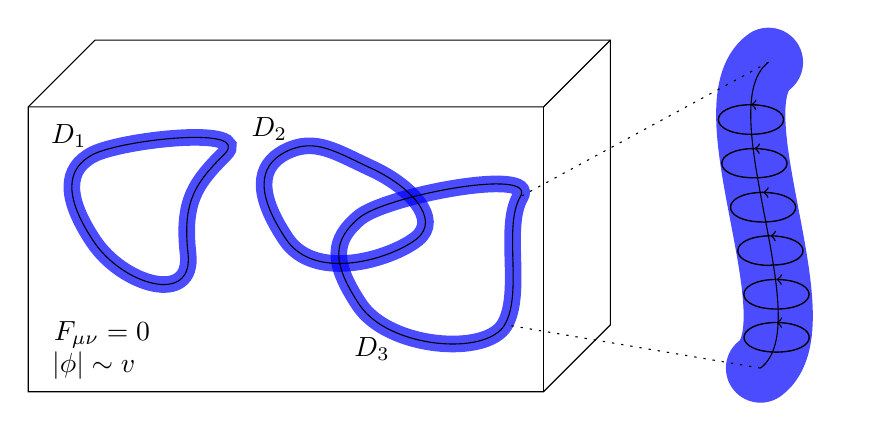
\begin{tikzpicture}[x=0.75pt,y=0.75pt,yscale=-0.7,xscale=0.7]

\draw   [color=blue ,draw opacity=0.7, line width=25, line cap = round] (551,249.25) .. controls (591,219.25) and (516.5,68.75) .. (556.5,38.75) ;
\draw    (551,249.25) .. controls (591,219.25) and (516.5,68.75) .. (556.5,38.75) ;

\draw   (47,69.5) -- (93,23.5) -- (447.67,23.5) -- (447.67,219.5) -- (401.67,265.5) -- (47,265.5) -- cycle ; \draw   (447.67,23.5) -- (401.67,69.5) -- (47,69.5) ; \draw   (401.67,69.5) -- (401.67,265.5) ;

\draw   [->][line width=0.5pt] (557.73,158.2) .. controls (527.89,158.61) and (527.89,178.45) .. (557.89,178.61)(557.89,178.36) .. controls (587.29,178.28) and (587.88,159.23) .. (557.73,158.2) ;
\draw   [->][line width=0.5pt]  (562,217.83) .. controls (532.17,218.25) and (532.17,238.08) .. (562.17,238.25) .. controls (591.57,237.92) and (592.15,218.87) .. (562,217.83);
\draw    [->][line width=0.5pt]  (561.91,188.2) .. controls (532.08,188.61) and (532.08,208.45) .. (562.08,208.61) .. controls (591.48,208.28) and (592.06,189.23) .. (561.91,188.2) ;
\draw    [->][line width=0.5pt]  (552.73,128.29) .. controls (522.89,128.7) and (522.89,148.54) .. (552.89,148.7) .. controls (582.29,148.37) and (582.88,129.32) .. (552.73,128.29) ;
\draw   [->][line width=0.5pt]  (546.73,98.11) .. controls (516.89,98.52) and (516.89,118.36) .. (546.89,118.27) .. controls (576.29,118.19) and (576.88,99.14) .. (546.73,98.11) ;
\draw   [->][line width=0.5pt]  (544.36,67.92) .. controls (514.53,68.34) and (514.53,88.17) .. (544.53,88.34) .. controls (573.93,88.01) and (574.52,68.96) .. (544.36,67.92) ;

\draw   [color=blue ,draw opacity=0.7, line width=6, line cap = round] (224.33,100.33) .. controls (244.33,90.33) and (258.33,100.33) .. (283.67,112) .. controls (309,123.67) and (331.67,146.67) .. (314.33,160.33) .. controls (297,174) and (244.33,190.33) .. (224.33,160.33) .. controls (204.33,130.33) and (204.33,110.33) .. (224.33,100.33) -- cycle ;
\draw   [color=blue ,draw opacity=0.7, line width=6, line cap = round] (275,145.67) .. controls (293,130.67) and (397.67,110.67) .. (385.67,131.33) .. controls (373.67,152) and (387.67,197.33) .. (375,219.33) .. controls (362.33,241.33) and (295,235.67) .. (275,205.67) .. controls (255,175.67) and (257,160.67) .. (275,145.67) -- cycle ;
\draw   [color=blue ,draw opacity=0.7, line width=6, line cap = round](92,102) .. controls (112,92) and (202,82) .. (182,102) .. controls (162,122) and (153,134.5) .. (157,170.5) .. controls (161,206.5) and (112,192) .. (92,162) .. controls (72,132) and (72,112) .. (92,102) -- cycle ;

\draw   (224.33,100.33) .. controls (244.33,90.33) and (258.33,100.33) .. (283.67,112) .. controls (309,123.67) and (331.67,146.67) .. (314.33,160.33) .. controls (297,174) and (244.33,190.33) .. (224.33,160.33) .. controls (204.33,130.33) and (204.33,110.33) .. (224.33,100.33) -- cycle ;
\draw   (275,145.67) .. controls (293,130.67) and (397.67,110.67) .. (385.67,131.33) .. controls (373.67,152) and (387.67,197.33) .. (375,219.33) .. controls (362.33,241.33) and (295,235.67) .. (275,205.67) .. controls (255,175.67) and (257,160.67) .. (275,145.67) -- cycle ;
\draw   (92,102) .. controls (112,92) and (202,82) .. (182,102) .. controls (162,122) and (153,134.5) .. (157,170.5) .. controls (161,206.5) and (112,192) .. (92,162) .. controls (72,132) and (72,112) .. (92,102) -- cycle ;

\draw  [dash pattern={on 0.84pt off 2.51pt}]  (556.5,38.75) -- (385.67,131.33) ;
\draw  [dash pattern={on 0.84pt off 2.51pt}]  (551,249.25) -- (375,219.33) ;

\draw (61,80) node [anchor=north west][inner sep=0.75pt]    {$D_{1}$};
\draw (199,75) node [anchor=north west][inner sep=0.75pt]    {$D_{2}$};
\draw (269.67,226.4) node [anchor=north west][inner sep=0.75pt]    {$D_{3}$};
\draw (63,215.4) node [anchor=north west][inner sep=0.75pt]    {$F_{\mu \nu } =0$};
\draw (61.67,236.4) node [anchor=north west][inner sep=0.75pt]    {$| \phi | \sim v$};
\end{tikzpicture}
\caption{Defects (blue closed lines) and their loci (black closed lines). On the right side of the picture, is represented in more detail the vortex associated to the defect $D_3$.}
\label{fig:defects-vortex}
\end{figure}

In order to understand how to ``open'' these line defects, let's first consider the restriction of the field strength $F$ of the vortex to a 2 dimensional disk crossing transversally the locus of the defect, such that the boundary of the disk identify the region where the configuration approximately approaches the vacuum one, as represented in fig.~\ref{fig:disk-defect}. 

\begin{figure}[h]
\centering

\tikzset{
pattern size/.store in=\mcSize, 
pattern size = 6pt,
pattern thickness/.store in=\mcThickness, 
pattern thickness = 0.3pt,
pattern radius/.store in=\mcRadius, 
pattern radius = 0pt}
\makeatletter
\pgfutil@ifundefined{pgf@pattern@name@EllipsePattern}{
\pgfdeclarepatternformonly[\mcThickness,\mcSize]{EllipsePattern}
{\pgfqpoint{0pt}{0pt}}
{\pgfpoint{\mcSize+\mcThickness}{\mcSize+\mcThickness}}
{\pgfpoint{\mcSize}{\mcSize}}
{
\pgfsetcolor{\tikz@pattern@color}
\pgfsetlinewidth{\mcThickness}
\pgfpathmoveto{\pgfqpoint{0pt}{0pt}}
\pgfpathlineto{\pgfpoint{\mcSize+\mcThickness}{\mcSize+\mcThickness}}
\pgfusepath{stroke}
}}
\makeatother
\tikzset{every picture/.style={line width=0.75pt}} %set default line width to 0.75pt        

\begin{tikzpicture}[x=0.75pt,y=0.75pt,yscale=-0.6,xscale=0.6]
%uncomment if require: \path (0,300); %set diagram left start at 0, and has height of 300

%Curve Lines [id:da33705367027161603] 
\draw   [color=blue ,draw opacity=0.7, line width=21, line cap = round] (571,269.25) .. controls (611,239.25) and (536.5,88.75) .. (576.5,58.75) ;
\draw   (571,269.25) .. controls (611,239.25) and (536.5,88.75) .. (576.5,58.75) ;

%Curve Lines [id:da21282626058718623] 
\draw   [->][line width=0.5pt] (577.73,178.2) .. controls (547.89,178.61) and (547.89,198.45) .. (577.89,198.61) .. controls (607.29,198.28) and (607.88,179.23) .. (577.73,178.2) ;
%Curve Lines [id:da8259045720854306] 
\draw   [->][line width=0.5pt] (582,237.83) .. controls (552.17,238.25) and (552.17,258.08) .. (582.17,258.25) .. controls (611.57,257.92) and (612.15,238.87) .. (582,237.83) ;
%Curve Lines [id:da00807708837653065] 
\draw   [->][line width=0.5pt] (581.91,208.2) .. controls (552.08,208.61) and (552.08,228.45) .. (582.08,228.36) .. controls (611.48,228.28) and (612.06,209.23) .. (581.91,208.2) ;
%Curve Lines [id:da9551996169478982] 
\draw  [->][line width=0.5pt]  (572.73,148.29) .. controls (542.89,148.7) and (542.89,168.54) .. (572.89,168.45) .. controls (602.29,168.37) and (602.88,149.32) .. (572.73,148.29) ;
%Curve Lines [id:da6438432478749674] 
\draw   [->][line width=0.5pt] (566.73,118.11) .. controls (536.89,118.52) and (536.89,138.36) .. (566.89,138.27) .. controls (596.29,138.19) and (596.88,119.14) .. (566.73,118.11) ;
%Curve Lines [id:da09026447567603135] 
\draw  [->][line width=0.5pt]  (564.36,87.92) .. controls (534.53,88.34) and (534.53,108.17) .. (564.53,108.34)(564.53,108.09) .. controls (593.93,108.01) and (594.52,88.96) .. (564.36,87.92) ;
%Shape: Ellipse [id:dp059940750148450794] 
\draw  [color=red][pattern=EllipsePattern, pattern color=red] [dash pattern={on 1pt off 0.5pt}, line width=0.5] (502.9,158.25) .. controls (502.9,136.16) and (534.24,118.25) .. (572.9,118.25) .. controls (611.56,118.25) and (642.9,136.16) .. (642.9,158.25) .. controls (642.9,180.34) and (611.56,198.25) .. (572.9,198.25) .. controls (534.24,198.25) and (502.9,180.34) .. (502.9,158.25) -- cycle ;

\draw (572.5,158.25) circle (1pt)[color=red, fill=red] ;

\end{tikzpicture}
\caption{Disk crossing the locus of the defect, whose boundary identify the region where the configuration approaches the vacuum.}
\label{fig:disk-defect}
\end{figure}

We then identify the points of the boundary to one-point, obtaining a closed 2-dimensional surface $S^2$ (topologically but with flat metric), as represented in fig.~\ref{fig:compactification-Riemann-sphere} (but for a plane, i.e. for an infinite radius of the disk, and for a sphere not only topological, but metric). 

\begin{figure}[h]
\centering
\def\svgwidth{\columnwidth}
\scalebox{0.45}{\adjustbox{trim={.0\width} {.15\height} {0.\width} {.32\height},clip}{\input{../img/riemann-sphere.pdf_tex}}}
\caption{Compactification of the plane by identification of the boundaries. Source: \url{https://demonstrations.wolfram.com/TheRiemannSphereAsAStereographicProjection/}}
\label{fig:compactification-Riemann-sphere}
\end{figure}

According to eq.~\eqref{eq:field-strength-vortex-magn-field} and eq.~\eqref{eq:integration-magnetic-field-vorticity}, integrating over such sphere (using spatial indices along the disk), we get
\begin{eq}\label{eq:vorticity-compact-disk-in}
	\frac1{2\pi}\int_{S^2}F_{ij}\de S^{ij} = n = \text{vorticity carried by the defect $D$}
\end{eq}
Let's see how $A_{i}$ behaves on such sphere. Using definition eq.~\eqref{eq:cov-der-vortex} and writing $\phi=|\phi|e^{i\theta}$, we get
\begin{eq}
	D_{i}\phi&=e^{i\theta}\partial_{i}|\phi|+|\phi|e^{i\theta}(e^{-i\theta}\partial_{i} e^{i\theta}-iA_{i})\\
	(D_{i}\phi)^*&=e^{-i\theta}\partial_{i}|\phi|+|\phi|e^{-i\theta}(e^{i\theta}\partial_{i} e^{-i\theta}+iA_{i})
\end{eq}
where we set $n_ee=1$ in order to get rid of these coefficients. Hence we obtained\todo{Come mai il secondo termine può esser singolare? É dovuto a possibili discontinuità di $\theta$ nel centro del vortice? In tal caso non sarebbe singolare anche il primo?}
\begin{eq}\label{eq:vortex-gauge-potential-singular-current}
	A_{i}=\underbrace{\vphantom{\int_T}\frac i2\frac{e^{-i\theta}D_{i}\phi-e^{i\theta}(D_{i}\phi)^*}{|\phi|}}_{\text{regular term}}+\underbrace{\vphantom{\int_T}\frac i2(e^{i\theta}\partial_{i} e^{-i\theta}-e^{-i\theta}\partial_{i} e^{i\theta})}_{\text{singular term}}
\end{eq}
where the first term is gauge-invariant, hence globally defined, and the curl of the second term is non-vanishing if and only if it is singular. 
Recall that $\theta(x)$ is an angle around the center of the vortex, where $|\phi|=0$. Without loss of generality we can assume that the center of the vortex coincide with the origin of the space. In the sense of distributions, the spatial components of the field strength of the singular term above is\footnote{The distribution $\delta_{|\phi|^{-1}(0)}( x)$ is made of a $\delta$-distributions centered at points of $|\phi|^{-1}(0)$.}
\begin{eq}
	\lctens^{ij}\partial_i\left(\frac i2(e^{i\theta}\partial_j e^{-i\theta}-e^{-i\theta}\partial_j e^{i\theta})\right)
	=\frac1i\lctens^{ij}\partial_i\partial_j\log e^{i\theta}=2\pi\,\delta_{|\phi|^{-1}(0)}(x)
\end{eq}
since the dependence of $\theta$ on the space coordinates goes with $\arctan\frac yx$. Hence such field strength is non zero (actually, singular) only in the center of the vortex. Therefore the spatial part of the field strength of $A_\mu$ is
\begin{eq}\label{eq:vortex-field-strength-transverse-plane}
	F_{ij}( x)=\partial_{[i}a_{j]}(x)+2\pi\,\delta_{|\phi|^{-1}(0)}(|\phi|)\lctens_{ij}
\end{eq}
where $a_\nu$ denotes some regular configuration. 

We see then that one can identify the locus of the defect in $F_{\mu\nu}$ in terms of a ``singular current'' (i.e. ``$\delta$-like'') having the support where $|\phi|$ vanishes, which is necessarily closed because the boundary condition at infinity is $|\phi|=v$. 

\subsubsection{Open defects}

If we want to open a defect and $ x$ is a boundary of the locus of such defect, we need to construct a 2-tensor $F_{\mu\nu}^{ x}$ such that for a metric (i.e. curved embedded in $\R^3$) 2-sphere $S_x^2$ centered at $x$ and of arbitrarily small radius we have\footnote{This is the same of eq.~\eqref{eq:vorticity-compact-disk-in}, assuming that there is no component along $x^0$ in ${S_{\vec x}^2}$.}
\begin{eq}
	\int_{S_{ x}^2}F_{\mu\nu}^{ x}\de y^\mu\de y^\nu=2\pi n
\end{eq}
and then if $B_{ x}^3$ is the ball centered in $ x$ whose boundary is $S^2_{ x}$, by Gauss theorem we have
\begin{eq}
	\int_{S^2_{ x}}F_{\mu\nu}^{ x}\de y^\mu\de y^\nu=\int_{B^3_{ x}}\lctens^{\mu\nu\rho}\partial_\mu F_{\nu\rho}^{ x}\de^3y=2\pi n
\end{eq}
which should hold for any arbitrarily small radius, so that
\begin{eq}\label{eq:condition-field-strength-vorticity}
	\lctens^{\mu\nu\rho}\partial_\mu F_{\nu\rho}^{ x}( y)=2\pi n\,\delta(x-y)
\end{eq}
or equivalently, using $\lctens^{\mu\nu\rho}F_{\nu\rho}^{x}=B^\mu_{x}$ where $B^\mu_{x}$ is the magnetic field centered at $x$, 
\begin{eq}\label{eq:vorticity-compact-disk-bc}
	\big(\nabla\cdot B_{ x}\big)( y)=2\pi n\,\delta( x- y)
\end{eq}
This is precisely the magnetic field of a \emph{monopole} in $\R^3$, i.e. the analogue of a point-like electric charge of charge $q$ which obeys
\begin{eq}
	\big(\nabla\cdot E_{ x}\big)( y)=q\,\delta( x- y)
\end{eq}
with the magnetic field replacing the electric field. 

Therefore we can build open defects constructing line defects with monopoles at the boundaries. With respect to fig.~\ref{fig:disk-defect}, this is equivalent to the introduction of two points at the boundaries of the line, describing classical monopoles, as represented in fig.~\ref{fig:open-defect-vortex}. Comparing eq.~\eqref{eq:vorticity-compact-disk-in} and eq.~\eqref{eq:vorticity-compact-disk-bc} we see that such monopoles ``provide the right vorticity'' to the defect. 

\begin{figure}[h]
\centering
\tikzset{every picture/.style={line width=0.75pt}}     
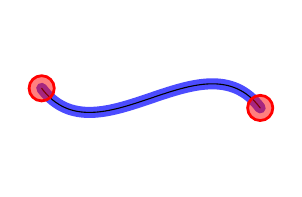
\begin{tikzpicture}[x=0.75pt,y=0.75pt,yscale=-0.9,xscale=0.9,rotate=90]

%Curve Lines [id:da8908477525317537] 
\draw   [color=blue ,draw opacity=0.7, line width=4, line cap = round] (31,141.5) .. controls (71,111.5) and (1.5,54.5) .. (41.5,24.5) ;
\draw   [line cap = round] (31,141.5) .. controls (71,111.5) and (1.5,54.5) .. (41.5,24.5) ;
%Shape: Circle [id:dp297621710933869] 
\draw  [color=red, line width=1, fill=red, fill opacity=0.5] (24.25,141.5) .. controls (24.25,137.77) and (27.27,134.75) .. (31,134.75) .. controls (34.73,134.75) and (37.75,137.77) .. (37.75,141.5) .. controls (37.75,145.23) and (34.73,148.25) .. (31,148.25) .. controls (27.27,148.25) and (24.25,145.23) .. (24.25,141.5) -- cycle ;
%Shape: Circle [id:dp807790352207095] 
\draw  [color=red, line width=1, fill=red, fill opacity=0.5] (34.75,24.5) .. controls (34.75,20.77) and (37.77,17.75) .. (41.5,17.75) .. controls (45.23,17.75) and (48.25,20.77) .. (48.25,24.5) .. controls (48.25,28.23) and (45.23,31.25) .. (41.5,31.25) .. controls (37.77,31.25) and (34.75,28.23) .. (34.75,24.5) -- cycle ;

\end{tikzpicture}
\caption{Representation of an open defect, whose boundaries are described by monopoles (red circles).}
\label{fig:open-defect-vortex}
\end{figure}

\subsubsection{Correlators}

Similarly to what we have done for the kink, where we modified the action introducing a new parallel transporter to construct the open defects, now we should insert classical monopole-antimonopole pairs at the points where we create and annihilated the quantum vortices of our theory. Correlators of the quantum vortex field will have insertion points at the monopoles positions. As usual, our construction can be made rigorous in the lattice approximation. 

%%%%%%%%%%%%%%%%%%%%%%%
%%%%%%%% LECTURE 19 %%%%%%%%
%%%%%%%%%%%%%%%%%%%%%%%

\skipline

Let $F_{\mu\nu}^{xy}$ be the field strength of a monopole at $ y$ ($n=1$) and a antimonopole ($n=-1$) at $ x$ and let $A_\mu^{xy}$ be the corresponding gauge potential. A possible choice for $F_{\mu\nu}^{xy}$ and $A_\mu^{xy}$ is the following. Let $\gamma_{xy}$ be a curve with boundary $ x$ and $ y$ in $\R^3$ oriented from $ y$ to $ x$ and define the current\footnote{This is the \emph{Poincaré dual} of $\gamma_{xy}$.}
\begin{eq}
	j_{\mu\nu}^{xy}( z):=\int_{\gamma_{xy}}\de w^\alpha\,\lctens_{\alpha\mu\nu}\delta( z- w)
\end{eq}
and we take
\begin{eq}\label{eq:field-strength-monopole-v}
	F_{\mu\nu}^{xy}( z)&:=-2\pi\int\de^3 w\,\partial^\alpha\Delta^{-1}( z- w)\,\half\partial_{[\alpha}j_{\mu\nu]}^{xy}( w)\\
	&=2\pi\int\de^3 w\,\partial^\alpha\Delta^{-1}( z- w)\lctens_{\alpha\mu\nu}[\delta( w- x)-\delta( w- y)]
\end{eq}
where $\Delta^{-1}( x)$ is the kernel of the inverse of the Laplacian in 3 dimensions, and in the second line we used Gauss theorem to evaluate the integral at the boundaries of $\gamma_{xy}$ (the change of sign is due to the orientation of $\gamma_{xy}$). 
For the gauge potential we can choose
\begin{eq}
	A_\mu^{xy}( z):=2\pi\int\de^3w\,\partial^\alpha\Delta^{-1}( z- w)j_{\alpha\mu}^{xy}( w)
\end{eq}

Let us check that $A_\mu^{xy}$ and $F_{\nu\rho}^{xy}$ really describe monopoles at the boundaries of the vortex, i.e. satisfy eq.~\eqref{eq:condition-field-strength-vorticity}, which reads
\begin{eq}
	\lctens^{\mu\nu\rho}\partial_\mu F_{\nu\rho}^{xy}( z)=2\pi \big(\delta( z- x)-\delta( z- y)\big)
\end{eq}
According to our definitions we have\footnote{From the second to the third line we used integration by parts together with
\begin{eq}
	\int\de^3w\,\Delta^{-1}( z- w)\partial_\alpha^{( w)}( w)=-\int\de^3w\,\partial_\alpha^{( w)}\Delta^{-1}( z- w)j( w)=\int\de^3w\,\partial_\alpha^{( z)}\Delta^{-1}( z- w)j( w)
\end{eq}
From the third to the fourth we exchanged the labels $\nu\leftrightarrow\rho$ in the third term and we used $\lctens^{\mu\nu\rho}=-\lctens^{\mu\rho\nu}$. From the fifth to the sixth we used $\partial^\alpha\partial_\alpha=-\Delta$ (according to our mostly minus signature), so that $\partial_\alpha\partial^\alpha\Delta^{-1}( z- w)=-\delta( z- w)$. 
}
\begin{eq}
	\lctens^{\mu\nu\rho}\partial_\mu F_{\nu\rho}^{xy}( z)
	&=-2\pi\lctens^{\mu\nu\rho}\partial_\mu\int\de^3 w\,\partial^\alpha\Delta^{-1}( z- w)\,\half\partial_{[\alpha}j_{\nu\rho]}^{xy}( w)\\
	&=-2\pi\lctens^{\mu\nu\rho}\partial_\mu\int\de^3 w\,\partial^\alpha\Delta^{-1}( z- w)\,\big(\partial_{\alpha}j_{\nu\rho}^{xy}( w)+\partial_{\nu}j_{\rho\alpha}^{xy}( w)+\partial_{\rho}j_{\alpha\nu}^{xy}( w)\big)\\
	&=-2\pi\lctens^{\mu\nu\rho}\partial_\mu\int\de^3 w\,\big(\partial_\alpha\partial^\alpha\Delta^{-1}( z- w)j_{\nu\rho}^{xy}( w)+\\
	&\hspace{2cm}+{\partial_{\nu}\partial^\alpha\Delta^{-1}( z- w)j_{\rho\alpha}^{xy}( w)+\partial_{\rho}\partial^\alpha\Delta^{-1}( z- w)j_{\alpha\nu}^{xy}( w)\big)}\\
	&=-2\pi\lctens^{\mu\nu\rho}\partial_\mu\int\de^3 w\,\partial_\alpha\partial^\alpha\Delta^{-1}( z- w)j_{\nu\rho}^{xy}( w)+\\
	&\hspace{2cm}+{\partial_{\nu}\partial^\alpha\Delta^{-1}( z- w)j_{\rho\alpha}^{xy}( w)-\partial_{\nu}\partial^\alpha\Delta^{-1}( z- w)j_{\alpha\rho}^{xy}( w)\big)}\\
	&=-2\pi\lctens^{\mu\nu\rho}\partial_\mu\int\de^3 w\,\partial_\alpha\partial^\alpha\Delta^{-1}( z- w)j_{\nu\rho}^{xy}\\
	&=2\pi\lctens^{\mu\nu\rho}\partial_\mu\int\de^3 w\,\delta( z- w)j_{\nu\rho}^{xy}( w)\\
	&=2\pi\lctens^{\mu\nu\rho}\partial_\mu\, j_{\nu\rho}^{xy}( z)\\[-4pt]
	&=2\pi\,\partial_\mu\, \int_{\gamma_{xy}}\de w^\alpha\,\overbrace{\lctens^{\mu\nu\rho}\lctens_{\alpha\nu\rho}}^{\delta^\mu_\alpha}\delta( z- w)\\
	&=2\pi\, \int_{\gamma_{xy}}\de w^\alpha\,\partial_\alpha\delta( z- w)\\
	&=2\pi\,\big(\delta( z- x)-\delta( z- y)\big)
\end{eq}
as we claimed. 
%
Now, let's derive the relation between $F_{\mu\nu}^{xy}$ and $A_\mu^{xy}$. One can write
\begin{eq}\label{eq:QFT-vertex-F-A-relation}
	F_{\mu\nu}^{xy}( z)&=-2\pi\int\de^3 w\,\partial^\alpha\Delta^{-1}( z- w)\,\half\partial_{[\alpha}j_{\mu\nu]}^{xy}( w)\\
	&=-2\pi\int\de^3 w\,\big(\partial_\alpha\partial^\alpha\Delta^{-1}( z- w)j_{\mu\nu}^{xy}( w)+\\
	&\hspace{2cm}+{\partial_{\mu}\partial^\alpha\Delta^{-1}( z- w)j_{\nu\alpha}^{xy}( w)+\partial_{\nu}\partial^\alpha\Delta^{-1}( z- w)j_{\alpha\mu}^{xy}( w)\big)}\\
	&=2\pi\,j_{\mu\nu}^{xy}( z)+\partial_\mu A_\nu^{xy}( z)-\partial_{\nu} A_\mu^{xy}( z)
\end{eq}
Hence the field strength of $A_\mu$ is equal to the usual curl of the gauge potential, $2\,\partial_{[\mu} A_{\nu]}^{xy}( z)$, up to a singular current $2\pi\,j_{\mu\nu}^{xy}( z)$. Such current is called \emph{Dirac string}, and was introduced by Dirac, in order to write the field strength of a monopole. 

From the calculation we see that $F_{\mu\nu}^{xy}$ is independent on the choice of $\gamma^{xy}$, i.e. of the Dirac string, it depends only on the boundary points. Therefore the Dirac string is an unphysical quantity. Indeed if we choose another curve $\gamma^{\prime{xy}}$ with the same boundaries as $\gamma^{xy}$, the difference $\gamma^{\prime{xy}}-\gamma^{xy}$ has no boundary, hence
\begin{eq}
	\lctens^{\mu\nu\rho}\partial_\mu(j_{\nu\rho}^{\prime{xy}}-j_{\nu\rho}^{xy})=0
	\tso
	j_{\nu\rho}^{\prime{xy}}-j_{\nu\rho}^{xy}=\partial_\nu\xi_\rho-\partial_\rho\xi_\nu
\end{eq}
with $\xi_\nu$ and integer current. But then
\begin{eq}
	\partial_{[\mu}A^{\prime{xy}}_{\nu]}( z)-\partial_{[\mu}A_{\nu]}^{xy}( z)
	&=2\pi\,\partial_{[\mu}\int\de^3w\,\partial^\alpha\Delta^{-1}( z- w)(j^{\prime{xy}}_{\nu]\alpha}( w)-j^{xy}_{\nu]\alpha}( w))\\
	&=2\pi\,\partial_{[\mu}\int\de^3w\,\partial^\alpha\Delta^{-1}( z- w)\partial_{\nu]}\xi_\alpha( w)-\\
	&\qquad-2\pi\,\partial_{[\mu}\int\de^3w\,\partial^\alpha\Delta^{-1}( z- w)\partial_{\alpha}\xi_{\nu]}( w)\\
	&=2\pi\int\de^3w\,\partial_{[\mu}\partial^\alpha\Delta^{-1}( z- w)\partial_{\nu]}\xi_\alpha( w)+\\
	&\qquad+2\pi\,\partial_{[\mu}\int\de^3w\,\partial^\alpha\Delta^{-1}( z- w)\cancel{\partial_{[\mu}\partial_{\nu]}}\xi_\alpha( w)-\\
	&\qquad-2\pi\,\partial_{[\mu}\int\de^3w\,\partial_{\alpha}\partial^\alpha\Delta^{-1}( z- w)\xi_{\nu]}( w)\\
	&=2\pi\int\de^3w\,\cancel{\partial_{[\mu}\partial_{\nu]}}\partial^\alpha\Delta^{-1}( z- w)\xi_\alpha( w)+\\
	&\qquad+2\pi\,\partial_{[\mu}\int\de^3w\,\delta( z- w)\xi_{\nu]}( w)\\
	&=2\pi\,\partial_{[\mu}\xi_{\nu]}( z)\\
	&=2\pi\big( j_{\mu\nu}^{\prime{xy}}( z)-j_{\mu\nu}^{xy}( z)\big)
\end{eq}
where in the second line $\alpha$ is not included in the antisymmetrization of the indices. Hence we see from eq.~\eqref{eq:QFT-vertex-F-A-relation} that $F_{\mu\nu}^{xy}$ is unchanged. 

From eq.~\eqref{eq:QFT-vertex-F-A-relation} we see also that $F_{\mu\nu}^{xy}$ has the same structure of the field strength of closed defects, eq.~\eqref{eq:vortex-field-strength-transverse-plane}, when restricted to the transverse plane. The difference is that now $j_{\mu\nu}$ has a boundary: the location of the monopole-antimonopole pairs. 

\skipline

Now we can come back to our vortex correlation function. We define the Euclidean modified Lagrangian (for $n_e=1$) by including terms associated to the monopoles
\begin{eq}
	\lag^{xy}=\frac1{4e^2}(F_{\mu\nu}+F_{\mu\nu}^{xy})^2+|(\partial_\mu-i(A_\mu+A_\mu^{xy}))\phi|^2+\lambda(|\phi|^2-v^2)^2+{\text{possible counterterms}\atop\text{and gauge fixing terms}}
\end{eq}
and, in the non-relativistic case case, we substitute
\begin{eq}
	|(\partial_0-i(A_0+A_0^{xy}))\phi|^2
	\quad\to\quad
	\phi^*(\partial_0-i(A_0+A_0^{xy}))\phi
\end{eq}
Moreover we denote by $S^{xy}$ the associated action. 
Notice that
\begin{eq}
	\int\de^3z\,F^{\mu\nu}F_{\mu\nu}^{xy}
	=\int\de^3z\,\partial^{[\mu}A^{\nu]}F_{\mu\nu}^{xy}
	=\int\de^3z\,\partial^{\mu}A^{\nu}F_{\mu\nu}^{xy}
	=-\int\de^3z\,A^{\nu}\partial^{\mu}F_{\mu\nu}^{xy}
	\overset{\eqref{eq:field-strength-monopole-v}}=0
\end{eq}
where we used $\partial^{\mu}F_{\mu\nu}^{xy}=0$, which follows directly from the definition eq.~\eqref{eq:field-strength-monopole-v}, and
\begin{eq}
	\int\de^3z\,(F_{\mu\nu}^{xy})^2
	&=(2\pi)^2\int\de^3z\,\de^3w\,\de^3\tilde w\,\partial^\alpha\Delta^{-1}( z- w)\lctens_{\alpha\mu\nu}[\delta( w- x)-\delta( w- y)]\times\\
	&\qquad\times\partial_\beta\Delta^{-1}( z- w)\lctens^{\beta\mu\nu}[\delta( {\tilde w}- x)-\delta( {\tilde w}- y)]\\
	&=(2\pi)^2\int\de^3z\,\de^3w\,\de^3\tilde w\,\partial^\alpha\Delta^{-1}( z- w)[\delta( w- x)-\delta( w- y)]\times\\
	&\qquad\times\partial_\alpha\Delta^{-1}( z- {\tilde w})[\delta( {\tilde w}- x)-\delta( {\tilde w}- y)]\\
	&=(2\pi)^2\int\de^3z\,\de^3w\,\Delta^{-1}( z- w)[\delta( w- x)-\delta( w- y)][\delta( {z}- x)-\delta( {z}- y)]\\
	&=(2\pi)^2\int\de^3z\,\big[\Delta^{-1}( z- x)-\Delta^{-1}( z- y)\big][\delta( {z}- x)-\delta( {z}- y)]\\
\end{eq}
where from the second to the third line we integrated by parts in $ z$ and then we used $\partial^\alpha\partial_\alpha\Delta^{-1}( z- {\tilde w})=-\delta( z- {\tilde w})$. The last line is clearly divergent since both $\int\de^3z\,\Delta^{-1}( z- x)\delta( {z}- x)$ and $\int\de^3z\,\Delta^{-1}( z- y)\delta( {z}- y)$ are divergent quantities. However, such divergent quantities do not depend on the spacetime points, hence can be eliminated with an appropriate counternterm.

Finally the 2-point correlation function of the vortex in the path integral formalism is given by
\begin{eq}
	\langle v_{+1}( x)v_{-1}( y)\rangle:=\left[\frac{\int\pide\phi\pide A\,e^{-S^{xy}}}{\int\pide\phi\pide A\,e^{-S}}\right]_{\text{ren}}
\end{eq}
where $[\ldots]_{\text{ren}}$ denote the previous renormalization and $v_{n}( x)$ denotes the vortex insertion at $ x$ with the monopole at $ x$ providing the vorticity $n$ of the vortex. 

One can generalize this construction to an arbitrary number of vortex insertions, provided that the total charge of the monopoles is zero. We can also include insertion of ordinary gauge invariant field, such as the electromagnetic field field strength of the Wilson loop. However such insertion need a modification with respect to the insertion in the vacuum, as it happened in the kinks case. For example,  in order to introduce the $ x,  y$ vortex insertion in a electromagnetic field correlator we should replace the electromagnetic field strength by
\begin{eq}
	F_{\mu\nu}
	\quad\to\quad
	F_{\mu\nu}+F_{\mu\nu}^{xy}
\end{eq}
or in the case of a Wilson loop $W_\alpha(\contour)$ with support on $\contour$, we should replace
\begin{eq}
	W_\alpha(\contour):=e^{\displaystyle i\alpha\oint_\contour A_\mu\de x^\mu}
	\quad\to\quad
	W_\alpha(\Sigma):=e^{\displaystyle i\alpha\left[\oint_\contour A_\mu\de x^\mu+\int_\Sigma F_{\mu\nu}^{xy}\de x^\mu\de x^\nu\right]}
\end{eq}
where $\Sigma$ is any surface such that $\partial\Sigma=\contour$. 

\subsubsection{The reconstructed QFT}

These correlators satisfy OS axioms and the reconstructed vortex field operator $\op v_n( x)$ satisfy
\begin{eq}
	\langle v_{+1}(x)v_{-1}(y)\rangle=\bra\Omega\op v_{-1}(\vec y)\,e^{-(x^0-\,y^0)t}\,\op v_{+1}(\vec x)\ket\Omega
\end{eq}
The Wilson loop operator $\op W_\alpha(\Sigma)$ reconstructed from $W_\alpha(\Sigma)$ can be used to define the topological charge $\op Q$ measuring the vorticity $n$ of the vortex. Indeed we define the $\op Q$ by
\begin{eq}
	e^{i\alpha2\pi\op Q}=\lim_{R\to\infty}\frac{\op W_\alpha(\contour_R)}{\bra\Omega\op W_\alpha(\contour_R)\ket\Omega}
\end{eq}
where $\contour_R$ is a circle of radius $R$ and time coordinate 0, and the limit is taken in the weak topology. Let $\Sigma_R$ be a flat surface bounded by $\contour_R$ and $r$ by the reflection in the Euclidean time 0 plane, and take $x^0>0,y^0>0$, then we have\todo{Qui è corretto $F_{\mu\nu}^{xy}$ o dovremmo avere $ry$ al posto di $y$? (questo risolverebbe alcuni dei problemi che ho riportato nel box successivo)}
\begin{eq}\label{eq:vortex-average-charge-op}
	\bra{\op v_1(y)\Omega}e^{i\alpha2\pi\op Q}\ket{\op v_1(x)\Omega}
	&=\lim_{R\to\infty}\frac{\displaystyle\langle v_{-1}(ry)\exp[ i\alpha\left(\oint_{\contour_R} A_\mu\de x^\mu+\int_\Sigma F_{\mu\nu}^{x(ry)}\de x^\mu\de x^\nu\right)] v_{+1}(x)\rangle}{\displaystyle\langle \exp[ i\alpha\oint_{\contour_R} A_\mu\de x^\mu] \rangle}\\
	&=\lim_{R\to\infty}\frac{\displaystyle\langle v_{-1}(ry)\exp[ i\alpha\left(\oint_{\contour_R} A_\mu\de x^\mu+2\pi\int_\Sigma j_{\mu\nu}^{x(ry)}\de x^\mu\de x^\nu\right)] v_{+1}(x)\rangle}{\displaystyle\langle \exp[ i\alpha\oint_{\contour_R} A_\mu\de x^\mu] \rangle}\\
	&=\exp[2\pi i\alpha\int_\Sigma j_{\mu\nu}^{x(ry)}\de x^\mu\de x^\nu]\frac{\displaystyle\cancel{\langle \exp[ i\alpha\oint_{\contour_R} A_\mu\de x^\mu] \rangle}\langle v_{-1}(ry)v_{+1}(x)\rangle}{\displaystyle\langle \cancel{\exp[ i\alpha\oint_{\contour_R} A_\mu\de x^\mu] \rangle}}\\
	&=e^{i\alpha2\pi n}\braket{\op v_1(y)\Omega}{\op v_1(x)\Omega}
\end{eq}
where from the first line to the second one we changed variable in the path integral of the numerator from $A$ to $\tilde A=A+A^{x(ry)}$, and from the second line to the third we used cluster property, as represented in fig.~\ref{fig:vortex-average-charge-op}. As it is clear from the figure, $\int_\Sigma j_{\mu\nu}^{x(ry)}\de x^\mu\de x^\nu$ equals the number of intersection between the curve $\gamma^{xy}$ and $\Sigma_R$ counted with signs depending on the orientation.

\begin{figure}[h]
\centering
\tikzset{
pattern size/.store in=\mcSize, 
pattern size = 6pt,
pattern thickness/.store in=\mcThickness, 
pattern thickness = 0.3pt,
pattern radius/.store in=\mcRadius, 
pattern radius = 0pt}
\makeatletter
\pgfutil@ifundefined{pgf@pattern@name@EllipsePattern}{
\pgfdeclarepatternformonly[\mcThickness,\mcSize]{EllipsePattern}
{\pgfqpoint{0pt}{0pt}}
{\pgfpoint{\mcSize+\mcThickness}{\mcSize+\mcThickness}}
{\pgfpoint{\mcSize}{\mcSize}}
{
\pgfsetcolor{\tikz@pattern@color}
\pgfsetlinewidth{\mcThickness}
\pgfpathmoveto{\pgfqpoint{0pt}{0pt}}
\pgfpathlineto{\pgfpoint{\mcSize+\mcThickness}{\mcSize+\mcThickness}}
\pgfusepath{stroke}
}}
\makeatother
\tikzset{every picture/.style={line width=0.75pt}} %set default line width to 0.75pt        
\begin{tikzpicture}[x=0.75pt,y=0.75pt,yscale=-0.8,xscale=0.8]
%Straight Lines [id:da766238486428902] 
\draw   [->] (120,200) -- (120,62) ;
\draw   [line width=0.5] (115,130) -- (125,130) ;

%Shape: Ellipse [id:dp6571871291563145] 
\draw  [pattern=EllipsePattern] (160,130) .. controls (160,118.95) and (245.07,110) .. (350,110) .. controls (454.93,110) and (540,118.95) .. (540,130) .. controls (540,141.05) and (454.93,150) .. (350,150) .. controls (245.07,150) and (160,141.05) .. (160,130) -- cycle ;

%Straight Lines [id:da718304516065198] 
\draw   [line width=0.5] (180,130) -- (142,130) ;
\draw [shift={(140,130)}, rotate = 360] [color=black][line width=0.5]    (10.93,-3.29) .. controls (6.95,-1.4) and (3.31,-0.3) .. (0,0) .. controls (3.31,0.3) and (6.95,1.4) .. (10.93,3.29)   ;
\draw   [line width=0.5] (520,130) -- (558,130) ;
\draw [shift={(560,130)}, rotate = 180] [color=black  ][line width=0.5]    (10.93,-3.29) .. controls (6.95,-1.4) and (3.31,-0.3) .. (0,0) .. controls (3.31,0.3) and (6.95,1.4) .. (10.93,3.29)   ;

\draw (99,46.9) node [anchor=north west][inner sep=0.75pt]    {$\tau $};
\draw (96.5,120.4) node [anchor=north west][inner sep=0.75pt]    {$0$};
\draw (350,100) circle (2pt)[fill=black] node [anchor=south west][inner sep=3pt]    {$x$};
\draw (350,170) circle (2pt)[fill=black] node [anchor=north west][inner sep=3pt]    {$ry$};
\draw (446,87.4) node [anchor=north west][inner sep=0.75pt]    {$\Sigma_R $};
\end{tikzpicture}
\caption{Representation of the limit in eq.~\eqref{eq:vortex-average-charge-op} in one dimension less. Arrows represent the limit $R\to\infty$. The ellipse is $\Sigma_R$ and is completely contained in the $\tau=0$ plane. As $R\to\infty$ it is clear that any line from $ry$ to $x$ intersects $\Sigma_R$ an odd number of times with pairs of opposite orientation.}
\label{fig:vortex-average-charge-op}
\end{figure}

\skipline

If the total sum of topological charge (vorticity) of the vortices in a correlator is non-vanishing, e.g. $n\in\Z^*$, we can define the correlator with a compensating charge $-n$ and send it to $\infty$, as in fig.~\ref{fig:combination-of-vorticities}. Since the mass of the vortex is finite, the contribution in the action of the defect associated to the compensating charge is infinite. This implies that all correlation functions with vanishing total charge are $0$, or in other wordk there are no coherent superposition of states with different total vorticity. Since these correlators can be interpreted as scalar products between states with quantum vortices in the reconstructed Hilbert space, this means that the Hilbert space obtained by OS reconstruction is splitted in superselection sectors, $\hs_n$, labelled by the total vorticity charge $n\in\Z$:
\begin{eq}	
	\hs=\bigoplus_{n\in\Z}\hs_n
\end{eq}

\begin{figure}[h]
\centering
\tikzset{every picture/.style={line width=0.75pt}} %set default line width to 0.75pt        

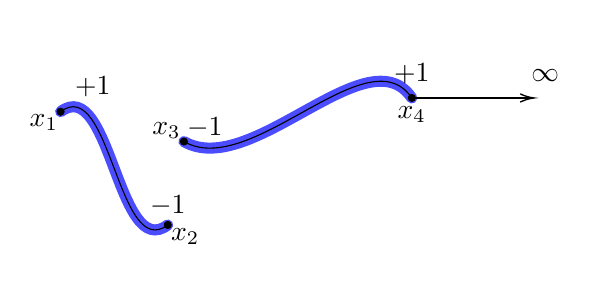
\begin{tikzpicture}[x=0.75pt,y=0.75pt,yscale=-0.6,xscale=0.6]
%Curve Lines [id:da778572141672087] 
\draw   [color=blue ,draw opacity=0.7, line width=4, line cap = round] (133,92.5) .. controls (173,62.5) and (179,213.5) .. (219,183.5) ;
%Curve Lines [id:da12345105516324217] 
\draw  [color=blue ,draw opacity=0.7, line width=4, line cap = round]  (232,116.5) .. controls (286,147.5) and (380,29.5) .. (415,81.5) ;
%Curve Lines [id:da778572141672087] 
\draw    (133,92.5) .. controls (173,62.5) and (179,213.5) .. (219,183.5) ;
%Curve Lines [id:da12345105516324217] 
\draw    (232,116.5) .. controls (286,147.5) and (380,29.5) .. (415,81.5) ;
%Straight Lines [id:da06469204048991184] 
\draw   [line width=0.5]  (415,81.5) -- (511,81.5) ;
\draw [shift={(513,81.5)}, rotate = 180][line width=0.5]    (10.93,-3.29) .. controls (6.95,-1.4) and (3.31,-0.3) .. (0,0) .. controls (3.31,0.3) and (6.95,1.4) .. (10.93,3.29)   ;

% Text Node
\draw (509,56.4) node [anchor=north west][inner sep=0.75pt]    {$\infty $};

\draw (133,92.5) circle (2pt)[fill=black] node [anchor=north east][inner sep=0.75pt]    {$x_1 $};
\draw (219,183.5) circle (2pt)[fill=black] node [anchor=north west][inner sep=1pt]    {$x_2 $};
\draw (232,116.5) circle (2pt)[fill=black] node [anchor=south east][inner sep=1pt]    {$x_3 $};
\draw (415,81.5) circle (2pt)[fill=black] node [anchor=north][inner sep=3pt]    {$x_4 $};

\draw (133,92.5) circle (2pt)[fill=black] node [anchor=south west][inner sep=5pt]    {$+1$};
\draw (219,183.5) circle (2pt)[fill=black] node [anchor=south ][inner sep=3pt]    {$-1$};
\draw (232,116.5) circle (2pt)[fill=black] node [anchor=south west][inner sep=1pt]    {$-1$};
\draw (415,81.5) circle (2pt)[fill=black] node [anchor=south][inner sep=5pt]    {$+1$};

\end{tikzpicture}
\caption{Representation of a system with total vorticity $-1$ (the charge in $x_4$ cannot be reached by any measure.}
\label{fig:combination-of-vorticities}
\end{figure}

One can prove (rigorously in the lattice approixmation) that actually $\op v(x)$ couple the vacuum to a one particle state, hence $\op v(x)$ create and annihilate vortex quantum particles. So there are really particles corresponding to vortices that we have seen, which can be created by scattering. They give a contribution in the spectrum of the Hamiltonian and in the non-relativistic framework they appear as ``quasi-particles''. In fact in superconductors the presence of these particles is evident because they modify \todo{Qua mi aveva fatto un annotazione che non ho capito bene dove andava collocata, spero di aver scritto correttamente} the spectral weight and possibly the dispersion relation of the other particles excitations. 

\skipline

Notice that all the above discussion was in absence of external magnetic field. If an external uniform magnetic field is introduced\footnote{Of curse in the thermodynamic limit it would need an infinite energy.} then the globally neutral gas of vortices discussed above turns into a gas with total vortex charge per unit area comparable with the uniform magnetic flux through that area.

\skipline

If we have no symmetry breaking of the global $U(1)$, both in the relativistic and the non-relativistic case, at the minima we have $|\phi|\sim0$ instead of $|\phi|\sim v$, and we have a condensation of defects reaching the infinity, making the additional defect from $x_3$ to $\infty$ in fig.~\ref{fig:combination-of-vorticities} invisible. So the Hilbert space of states cannot be splitted into superselection sectors and 
\begin{eq}
	\hs=\hs_0
\end{eq}
and the presence of vortices is completely irrelevant. 

\end{document}